%Template for a Computer Science Tripos Part II project dissertation
\documentclass[12pt,a4paper,twoside,openany]{report} \usepackage[pdfborder={0 0 0}]{hyperref}    % turns references into hyperlinks 
\usepackage[left=20mm, right=20mm, bottom=20mm, top=20mm]{geometry}  % adjusts page layout
\usepackage{karnaugh-map} 
\usepackage{pgf}
\usepackage{algorithm} 
\usepackage{algpseudocode} 
\usepackage{tikz} 
\usepackage{graphicx}
% allows inclusion of PDF, PNG and JPG images 
\usepackage{bm} 
\usepackage{listings} \usepackage{titlesec}
\usepackage{subcaption} \usepackage{array} \usepackage{verbatim} \usepackage{mathdots} \usepackage{amsfonts}
\usepackage{amssymb} \usepackage{xcolor} \usepackage{placeins} \usepackage{amsthm} \usepackage{amsmath}

\usepackage{tabu} 
\usepackage{docmute}   % only needed to allow inclusion of proposal.tex 
\usepackage[utf8]{inputenc} \usepackage{mathtools} \usepackage{changepage} \usepackage{url} \usepackage{blindtext} \usepackage{tabularx,booktabs}
\usepackage{dirtree} \usepackage{cite} \usepackage{float} % Prevent Latex from repositioning tables
\usepackage{graphicx}
\usepackage{listings}

\lstset{ language=Haskell, basicstyle=\linespread{1} \ttfamily\footnotesize, keywordstyle=\color{blue}, commentstyle=\color{gray}, stringstyle=\color{orange}, showstringspaces=false, breaklines=true,
  frame=lines,
  rulecolor=\color{gray},
  numbers=left, numberstyle=\tiny\color{gray}, xleftmargin=2em, framexleftmargin=1.5em, aboveskip=1em, belowskip=1em, escapeinside={(*}{*)}, captionpos=b }

% lstset{ language=Haskell, basicstyle=\ttfamily\small, breaklines=true, frame=single, numbers=left,
% numberstyle=\tiny\color{gray}, showstringspaces=false }

% \algrenewcommand\algorithmicrequire{\textbf{Input:}}
\algrenewcommand\algorithmicensure{\textbf{Output:}}
%--- Remove hbox warning
%----------------------------------------------------------------------------------------

% Formatting Commands
\newcommand{\keyword}[1]{\textbf{#1}} \newcommand{\tabhead}[1]{\textbf{#1}} \newcommand{\code}[1]{\texttt{#1}}
\newcommand{\file}[1]{\texttt{\bfseries#1}} \newcommand{\option}[1]{\texttt{\itshape#1}}

%----------------------------------------------------------------------------------------
%% *****************************************************************
\newlength{\upBranch} % shift up the text  lines <<<< 
\setlength{\upBranch}{0.7ex} % 


\newlength{\tolineSpace} % blank space bellow text  lines  <<< 
\setlength{\tolineSpace}{1mm}% 

\usepackage{xpatch} % needed <<<<<<<< 
\makeatletter

\DeclareMathOperator*{\argmax}{arg\,max} \DeclareMathOperator*{\argmin}{arg\,min}

\xpatchcmd{\dirtree} % root 
{\vbox{\@nameuse{DT@body@1}}} {\raisebox{-\tolineSpace}{\vbox{\@nameuse{DT@body@1}}}} {}{}    

\xpatchcmd{\dirtree} % below space 
{\advance\dimen\z@ by-\@nameuse{DT@lastlevel@\the\DT@countiv}\relax}
{\advance\dimen\z@ by-\tolineSpace \advance\dimen\z@ by-\@nameuse{DT@lastlevel@\the\DT@countiv}\relax} {}{}
    
\xpatchcmd{\dirtree}% shift up the text  lines 
{\kern\DT@sep\box\z@\endgraf}
{\kern\DT@sep\raisebox{-\upBranch}{\box\z@}\endgraf} {}{}    

\makeatother
%% *****************************************************************
\titleformat{\chapter}[display]
{\normalfont\huge\bfseries}{Chapter \thechapter}{1ex}
{\vspace{1.5ex}\Huge}
[\vspace{1.5ex}{\titlerule}]

% \titleformat{\chapter}
% {\normalfont\huge\bfseries}{\chaptertitlename\ }{0pt}{\Huge}[{\titlerule[0.8pt]}]
% {\normalfont\Large\bfseries}{\thesection}{1em}{}
%----- Language setting

\usepackage[english]{babel}

% \usepackage{silence}
% \WarningFilter{latex}{Overfull \hbox} 
% heheehe


\raggedbottom                           % try to avoid widows and orphans
\sloppy \clubpenalty1000% \widowpenalty1000%

\renewcommand{\baselinestretch}{1.05}    % adjust line spacing to make
% more readable


\theoremstyle{definition} \newtheorem{definition}{Definition}[section]

\graphicspath{{figs/}}

\begin{document}

\hbadness=10000
\hfuzz=10000pt


% Change these

\newcommand{\mcandidate}{2200D}
\newcommand{\mfullname}{Judah Daniels}
\newcommand{\mcollege}{Clare College}
\newcommand{\mtitle}{Inferring Harmony from Free Polyphony}
\newcommand{\ntitle}{Inferring Harmony from Free Polyphony}
\newcommand{\mexamination}{Computer Science Tripos -- Part II}
\newcommand{\mdate}{July, 2023}
\newcommand{\moriginator}{Christoph Finkensiep}
\newcommand{\msupervisor}{Dr Peter Harrison}
\newcommand{\mwordcount}{5434}
\newcommand{\mlinecount}{2272}
% Consent to the dissertation made available to University members
\newcommand{\mconsent}{I am content for my dissertation to be made available to the students and staff of the University.}
% For the Declaration of originality
\newcommand{\msignature}{Judah Daniels}


\bibliographystyle{acm}


\setlength{\parskip}{10pt} \setlength{\parindent}{0pt}

%%%%%%%%%%%%%%%%%%%%%%%%%%%%%%%%%%%%%%%%%%%%%%%%%%%%%%%%%%%%%%%%%%%%%%%%
% Title
%%%%%%%%%%%%%%%%%%%%%%%%%%%%%%%%%%%%%%%%%%%%%%%%%%%%%%%%%%%%%%%%%%%%%%%%

\thispagestyle{empty}

\rightline{\LARGE \textbf{\mfullname}}

\vspace*{60mm} \begin{center} \Huge \textbf{\mtitle} \\[5mm] \mexamination \\[5mm] \mcollege \\[5mm] \mdate  % today's date 
\end{center}

%%%%%%%%%%%%%%%%%%%%%%%%%%%%%%%%%%%%%%%%%%%%%%%%%%%%%%%%%%%%%%%%%%%%%%%%%%%%%%
% Proforma, table of contents and list of figures
%%%%%%%%%%%%%%%%%%%%%%%%%%%%%%%%%%%%%%%%%%%%%%%%%%%%%%%%%%%%%%%%%%%%%%%%%%%%%%

% \pagestyle{plain}
\pagenumbering{roman}

\newpage \newpage \section*{Declaration of originality}

I, \mfullname{} of \mcollege, being a candidate for Part II of the Computer Science Tripos, hereby declare that this
dissertation and the work described in it are my own work, unaided except as may be specified below, and that the
dissertation does not contain material that has already been used to any substantial extent for a comparable purpose.
\mconsent

\bigskip \leftline{Signed \msignature} \bigskip \leftline{Date \today}

\chapter*{Proforma}


{\large \begin{tabular}{ll} Candidate Number:   & \bf \mcandidate                   \\ Project Title:      & \bf \mtitle
    \\ Examination:        & \bf \mexamination, \mdate         \\ Word Count:         & \bf \mwordcount\footnotemark[1]
    \\ Code Line Count:    & \bf \mlinecount\footnotemark[2]   \\ Project Originator: & \bf \moriginator
    \\ Supervisor:         & \bf \msupervisor                  \\ \end{tabular} }

    \footnotetext[1]{This word count was computed by \texttt{texcount -v1 -sum -sub=chapter main.tex} } \footnotetext[2]{This code line count
    was computed by using \texttt{cloc} } \stepcounter{footnote}

    \section*{Original Aims of the Project}
    % The original aim was to implement a parsing algorithm for symbolic music, using the derivation to infer the
    % underlying harmonic structure, then explore data driven approaches for heuristic design.


    \section*{Work Completed}



    \section*{Special Difficulties} There were no special difficulties encountered in this project

    \newpage { \renewcommand{\baselinestretch}{0.75}\normalsize \tableofcontents
    \renewcommand{\baselinestretch}{1.0}\normalsize }
    % \listoffigures

    \newpage \section*{Acknowledgements} I'd like to thank Christoph Finkensiep and Peter Harrison for being awesome.



%%%%%%%%%%%%%%%%%%%%%%%%%%%%%%%%%%%%%%%%%%%%%%%%%%%%%%%%%%%%%%%%%%%%%%%
    % now for the chapters

    \pagestyle{headings}

    % \textit{This dissertation explores efficient search strategies for parsing symbolic music data using a musical
    % grammar for Automatic Chord Estimation (ACE). We first present a naive implementation of a parsing algorithm based
    % on a recent grammatical model, then address problems of intractability through classical heuristic search methods.
    % We will see that that my novel heuristic search algorithm achieves commendable results, providing a strong
    % foundation for a more sophisticated automated analysis system. }

    % \section{Motivation and Aim}
    % ACE usually assumes a small, finite set of chord types, but each chord can be expressed in
    % a practically infinite number of ways. 


    % \begin{figure}[h] \centering \begin{subfigure}[t]{\textwidth}
    % \centering\includegraphics[keepaspectratio,width=\textwidth]{intro/overview/generation.png} \caption{Modelling}
    % \label{fig:modellingOverview} \end{subfigure} \begin{subfigure}[t]{\textwidth}
    % \centering\includegraphics[keepaspectratio,width=\textwidth]{intro/overview/inference.png} \caption{Inference}
    % \label{fig:inferenceOverview}
    %   \end{subfigure} \caption{Problem overview} \label{fig:overview} \end{figure}

    
    % In this project, we consider a symbolic abstraction of a piece of music.
    % as a sequence of pitch instances with timing information.

    %, which together define the underlying harmony.
    % which describe units of harmony within 
    % $L = l_0, \dots, l_n$, by finding the sequence of labels $\hat{L}$ which
    
    % Harmony is a cognitive phenomenon that emerges as notes of different pitches sound simultaneously, wherein
    % collections of notes . 
    % Chord labels describe a high level property of the  used to describe a higher level 
    % These notes are divided into segments, which can each be described by a single chord label.
    % only two elements of the input piece into consideration, the pitches.
    % , a symbolic representation of a piece of music described by a sequence of pitch instances with timing information, we wish to

    % Novel ways to understand harmonic structure are sought after by music theorists, aiding the analysis and
    % composition of pieces. 


    % can be described using a sequence of chords, representing the higher level harmonic
    % structure of a piece. 
    % Given a surface $S$, we wish to infer a sequence of underlying chord labels $L = l_0, \dots, l_n$, 
    % by finding the sequence $\hat{L}$ which maximises the conditional probability of $L$ given $S$, which can
    % be expressed as:
    %
    % \begin{equation} \begin{aligned} \hat L &= \argmax_L P(L|S) \end{aligned} \end{equation} 
    % This reduction maps the set of surfaces to the set of reduced forms of each surface, denoted as $S \to
    % \mathcal{R}(S)$. 
    % In this mapping, each chord segment in the reduced surface comprises a subset of the notes in the corresponding original surface. 

    % This not providing an interpretable and explainable framework for inferring chord labels from a musical surface. 

    % The proposed project addresses the limitations of existing ACE approaches by developing a novel system that integrates the protovoice model with a chord segment reduction process.

    % Western tonal music often relies on sequences of chords to represent its harmonic structure. 
    % Automatic Chord Estimation (ACE) aims to infer these sequences from a piece of music. 
    % , providing an interpretable and explainable framework for inferring chord
    % labels. 

    % The protovoice model is a generative model that represents a musical piece as a result of recursively applying primitive operations on notes, forming a hierarchical structure encoding explicit relations between all the notes in a piece. The integration of the protovoice model with a chord segment reduction process provides an interpretable and explainable framework for inferring chord labels, uniquely inferring a sequence of chord labels along with an explicit explanation of how those labels relate to the surface.

    % Broadly, this project aims implements a novel approach to ACE in line with the development of
    % \textit{eXplainable Machine Learning}(XML) and \textit{Interpretable Machine Learning}(IML) models. 
      % \item An informed bottom-up heuristic that estimates the relative plausibility of each reduction step, which
      %   is used to improve the relative plausibility of the protovoice derivations. 
      % \item A stochastic search algorithm that efficiently explores the exponential parsing state-space, making use
      %   of the heuristic while carefully handling the trade-off between exploration and exploitation.

    % and mitigates designed to deal with the exponential state-space.
    % which explores the trade-offs between exploration and exploitation.
    % How can the relative plausibilities of a set of protovoice derivations be determined?
    % How should the exponential parsing state-space be dealt with?


    % The protovoice model offers a novel approach that unifies three
    % aspects of tonal music analysis that are traditionally considered independently. Voice-leading refers how notes
    % relate to each other \textit{sequentially} through time, while harmony emerges from the simultaneous interaction
    % between notes. Note \textit{function} how notes relate to each other through recursive \textit{functional
    % dependencies}. Previous models have been developed alongside inference algorithms to perform automatic chord
    % estimation that consider these dimensions of musical structure separately \cite{maxwellExpertSystemHarmonizing1995}
    % \cite{winogradLinguisticsComputerAnalysis1968}, but the protovoice is the first to model free polyphony, one of the
    % least restrictive forms of Western tonal music, and does so at a granular level. 
    % this is the first to provide a complete explanation of a piece of music at such a low level.

    % \cite{pardoAlgorithmsChordalAnalysis2002} utilise templates for each chord label, predicted the label for each
    % segment by computiting a numerical measure of proximity to the nearest template 
    % system created by McLeod includes a number of neural \textit{A Modular System for the Harmonic Analysis of Musical Scores using a Large Vocabularly}
    % \cite{mcleodModularSystemHarmonic2021} extract a set features from the input score .... Symbolic approaches ..... . 
    % One recent harmony analysis model consists of a combination of submodels
    % \cite{niEndtoendMachineLearning2011} \cite{mcleodModularSystemHarmonic2021}
    % \cite{masadaChordRecognitionSymbolic2018}. 

    % The need for explainable AI models has been raised \cite{}. For in order for. Consistentcy etc. Trust. 

    % This process can be reversed by \textit{parsing} a piece of music according to the
    % grammar described by the model, resulting in a list of possible \textit{derivations}, that is, a list of all the
    % ways the piece of music could have been produced through the recursive application of these simple rules. 
    % a list of descriptive chord labels, along with an explicit explanation of the underlying note-level structure.

    % by explaining how 
    % such that the parsing procedure results in a reduction of the original piece, $S \to \mathcal{R}(S)$. 

    % that can in turn be used to infer

    % abstract explanation of the underlying structure of a piece. 

    % a latent structure of a piece can be inferred. \cite{finkensiepModelingInferringProtovoice2021}. or a ne
    % applications, such as that encodes the recursive and hierarchical dependencies between notes, giving rise to
    % a grammar-like hierarchical system This model can be used to simplify a piece into a hierarchical structure which
    % encodes an understanding of the tonal/harmonic relations.

    % Finkensiep suggests in his thesis that the protovoice model may be an effective way to infer higher level latent
    % entities such as harmonies. Thus, in this project I will answer the question: is this model an effective way to
    % annotate harmonies? By ‘effective’ we are referring to two things: \begin{itemize} \item Accuracy: can the model
    % successfully emulate how experts annotate harmonic progressions in musical passages? \item Practicality: can the
    % model be used to do this within a reasonable time frame?
    % \end{itemize}



    % The problem of automated chord estimation has been subject to attention since the 80s, with handcrafted
    % grammar/rule-based being. 

    % Automatic chord estimation systems first emerged in in the 60's, utilising handcrafted grammar/rule-based systems
    % \cite{maxwellExpertSystemHarmonizing1992} \cite{winogradLinguisticsComputerAnalysis1968}, followed by the
    % development of optimisation algorithms in the early 2000s \cite{pardoAlgorithmsChordalAnalysis2002}. In more recent
    % years, supervised learning approaches have have risen in popularity, exploiting large datasets and improved compute
    % power \cite{niEndtoendMachineLearning2011} \cite{mcleodModularSystemHarmonic2021}
    % \cite{masadaChordRecognitionSymbolic2018}. \par The protovoice model offers a novel approach that unifies three
    % aspects of tonal music analysis that are traditionally considered independently. Voice-leading refers how notes
    % relate to each other \textit{sequentially} through time, while harmony emerges from the simultaneous interaction
    % between notes. Note \textit{function} how notes relate to each other through recursive \textit{functional
    % dependencies}. Previous models have been developed alongside inference algorithms to perform automatic chord
    % estimation that consider these dimensions of musical structure separately \cite{maxwellExpertSystemHarmonizing1995}
    % \cite{winogradLinguisticsComputerAnalysis1968}, but the protovoice is the first to model free polyphony, one of the
    % least restrictive forms of Western tonal music, and does so at a granular level. 
    % this is the first to provide a complete explanation of a piece of music at such a low level.

    % but in this project we use the relationship between these dimensions of music as the basis of heuristic design.
    % Distinction to be drawn between approaches that take segmented or non-segmented pieces. Some models make use of
    % a joint segmentation and labelling approach \cite{masadaChordRecognitionSymbolic2018}. 
    % \begin{itemize}
    %   \item Adapt and expand the protovoice parser to reduce a given surface up to the chord-tone level
    %   \item Implement a harmony model to infer the sequence of chord labels from the reduced surface
    %   \item Create a generalised framework for the 
    % \end{itemize}

    % I've shown that the protovoice model can be used to perform harmonic inference.

    % Through the synergy of an extremely 


    % In this project I present a \textbf{novel solution}, the \textbf{ProtoVoice Harmony Model (PVHM)} 

    % The \textbf{PVHM} uses \textit{heuristic search} strategies to infer \textit{latent structure} using the
    % protovoice model, followed by \textit{feature extraction} which finally allows the chord labels to be inferred
    % using a \textit{probabilistic model of harmony}.

    % This was an ambitious project; I met all the Success Criteria and completed the extension tasks. I show that the
    % protovoice model can be used to effectively annotate pieces with chord labels, and these results provide a promising
    % foundation for the model being developed further as a sophisticated tool for the automated analysis of western total
    % music. The PVHM has been made \textbf{open source} to accommodate future research in the area.
    %
    % Furthermore, the contribution of this project is not limited to ACE, but more broadly 

      % I first clarify the exact formulation of the task at hand, describing the general
      % challenges of ACE. I subsequently provide an exposition of the Protovoice Model, describing how it can be used to infer harmony in an interpretable manner. After a brief description of the probabilistic foundations of the project, I 
% , 
% including learning many features of Haskell such as monad transformers. 
% This was non-trivial and required me to learn about many features of Haskell, such as monad transformers 

% implementing an adaptation of this parser that
% allows it to be used by different algorithms, a harmony model and a number of algorithms used to perform reductions.
% and extending this parser so that 
% , as learning these
%
% empirically observed distributions of which notes appear depending on
% the chord label.
% I also make use of learned parameters from the implementation of the paper
% parameters would be beyond the scope of this project. 

      % . Subsequently, I discuss probabilistic programming and Bayesian inference, including a probabilistic
    % model of harmony. 
  % }

% We denote the protovoice reduction transformation as $f_{pv}:(\mathcal{S}, \Phi) \to (\mathcal{S'})$. We then consider
% computing $p(S'|L;\phi)$. $S'$ is the reduced surface. In order to be able to use this transformed representation,
% there is a constraint that $\argmax_L p(S'|L') \approxeq \argmax_L p(S|L)$. That is, after applying the transform, the
% maximum likelihood estimate of the reduced surface given each sequence of labels should be the same, or as close as
% possible to that of the unreduced surface. In other words, the solution should be \textit{invariant} or
% \textit{approximately invariant} to this transformation.
    % \setcounter{page}{1}
    \clearpage
    \pagenumbering{arabic}
    \thispagestyle{empty}
    \chapter{Introduction}
    The problem of inferring the harmonic structure of a piece of music, represented by a sequence of chords, is
    a fundamental task in the analysis and understanding of Western tonal music. Free polyphony refers to one of the
    most general forms of western music, wherein multiple independent melodic lines (or voices) are combined without
    adhering to strict rules or constraints. 
    % lines that are free to begin, end or meet together at any point.
    Symbolic approaches to Automatic Chord Estimation (ACE) usually solve such problems by taking a sequence of notes
    as the input, and generating a sequence of chord labels as the output.
    In this project, the input, called the \textit{surface}, is a sequence of notes with precise descriptions of when each note begins (onset) and ends (offset). 
    The output is a sequence of chord labels, each describing a \textit{chord segment}, a group of notes
    that sound simultaneously or in close succession. 

    % Automatic Chord Estimation has both theoretical and practical applications. 
    % Analysis of music often starts with the manual labeling of each chord, which is a time consuming and cognitively
    % demanding expert task. Sequences of chord labels provide compact representations for use in analysis, music identification
    % and music similarity finding \cite{masadaChordRecognitionSymbolic2018}. More broadly speaking, any system that
    % involves the understanding of written tonal music will benefit from chord estimation. 

    This project proposes a novel approach to ACE that integrates the proto-voice model \cite{finkensiepModelingInferringProtovoice2021}, a recent model of note-level structure, 
    with a chord segment reduction process. This contributes an \textbf{interpretable} framework for
    inferring sequences of chord labels by providing an explicit explanation of how those labels relate to the
    surface notes. Furthermore, I design and implement a \textbf{novel fitness function} and \textbf{efficient
      heuristic search
    algorithms} to improve on the computational complexity of the parsing algorithm provided in the proto-voice paper
    \cite{finkensiepModelingInferringProtovoice2021} from \textbf{exponential to linear time} with respect to the length
    of the piece.

    \section{Previous Work}

    Automatic chord estimation systems have ranged from handcrafted grammar/rule-based approaches
    \cite{maxwellExpertSystemHarmonizing1992} \cite{winogradLinguisticsComputerAnalysis1968}, to the
    development of optimisation algorithms \cite{pardoAlgorithmsChordalAnalysis2002}. 
    In more recent years, deep learning methods have risen in popularity, exploiting large datasets and improved compute
    power. Examples of deep architectures used include recurrent neural networks (RNNs)
    \cite{chenFunctionalHarmonyRecognition2018a} and long short-term memory (LSTM)
    networks \cite{dengLargeVocabularyAutomatic2018}. Some systems also make use of audio rather than symbols as an
    input, utilising
    convolutional neural networks (CNNs), and most recently convolutional recurrent neural networks (CRNNs)
    \cite{wuAutomaticChordEstimation2019} \cite{fardAutomaticChordRecognition2020}. These architectures have
    found success due to their ability to capture temporal dependencies in the music.

    A broad limitation of these existing ACE approaches is that they do not specify the precise relationship
    between the surface and the inferred chord labels. Deep-learning approaches
    typically involve a black box inference of the chord labels based on the raw input. For example, a recent chord classification model described by McLeod
    \cite{mcleodModularSystemHarmonic2021} consists of a neural network that takes a sequence of notes represented as
    one-hot feature vectors and outputs a distribution over a set of 1540 chord labels.
    Earlier probabilistic optimisation approaches consider the surface as being generated by a noisy process. Pardo and
    Birmingham's influential algorithm compares the notes in each segment to a set
    of templates describing common chords \cite{pardoAlgorithmsChordalAnalysis2002}. There is no explicit
    relationship described between the notes in each segment and the nearest template.

    The recent paper \textit{Modeling and Inferring Proto-voice Structure in Free
    Polyphony}\cite{finkensiepModelingInferringProtovoice2021} presents the proto-voice model, a generative model that
    represents a musical piece as a result of recursively applying primitive operations on notes. 
    The combination of these operations forms a hierarchical structure which encodes explicit relations
    between all the notes in a piece. 
    The paper presents a \textit{chart parsing} algorithm which can parse a piece of music according to the grammar
    outlined by the model, returning a list of possible
    \textit{derivations}, that is, all the ways the piece of music could have been created through the recursive application of these simple rules. 

    In this project, I build upon the proto-voice model by creating a new \textit{proto-voice harmony parser} to enable the generation of a \textit{reduction} of the musical
    surface that can be used to directly infer chord labels. In music analysis, a reduction refers to the process
    of simplifying a complex musical surface to reveal its underlying harmonic structure. 
    The new parser is used to reduce the piece, with the goal of finding a reduction that preserves the harmony of
    the piece, while eliminating extraneous notes. This reduction facilitates the inference of descriptive chord labels and provides an
    \textit{explicit explanation} through the corresponding proto-voice derivation, which has not been attempted before. 

    While the chart parsing algorithm provided \cite{finkensiepProtovoicesModelTonal2021} could in theory be used to
    generate harmonic annotations, the naive exhaustive parse strategy would be prohibitively time-consuming in
    practice for all but the shortest musical extracts; one half measure can have over 100,000 valid derivations
    \cite{finkensiepStructureFreePolyphony2023}. Moreover, not all derivations are created equally. Each one
    corresponds to a specific interpretation of the note-level structure within a given piece of music. These
    reductions align with intuitive or theoretical musical interpretations to differing extents, with most being implausible. 
    Determining the relative plausibility of derivations remains an \textit{open question}. 

    I provide answers to these questions by proposing and implementing a \textbf{novel heuristic fitness function} for
    proto-voice derivations and address the \textbf{exponential search space} using heuristics and pruning
    techniques to significantly reduce the time and space complexity from $\bm{\mathcal{O}(2^{n \cdot m})}$
      to $\bm{\mathcal{O}(n \cdot m)}$, where $n$ is the length of in piece and $m$ is the number of notes in each segment. 

    \section{Contributions of my Project}

    % The implementation of this project provides solutions to two open problems. The first is the question of how the relative plausibilities of protovoice derivations should be determined, and second is how to deal with the exponential parsing state-space.
    %

    The implementation of this project achieved all of the original aims. In doing so, the key contributions include:
    \begin{enumerate}
      \item Developing a novel approach to Automatic Chord Estimation that integrates the proto-voice model with
        a chord segment reduction process (Section~\ref{chap:implementation}). This not only provides an interpretable and explainable
        framework for Automatic Chord Estimation but also has the potential to contribute to a more comprehensive
        understanding of the underlying structure of Western tonal music. 
      \item Proposing and implementing an informed heuristic-based fitness function to evaluate proto-voice
        derivations, which decomposes into a estimated score for each reduction step (Section~\ref{sub:heuristicDesign}). This enables the identification of musically meaningful interpretations of the piece while discarding implausible derivations. 
      \item Designing and developing the proto-voice harmony parser which can generate reductions of the musical surface
        to facilitate chord label inference (Section~\ref{sec:protovoiceHarmonyParser}). 
        This has the benefit over previous approaches of providing an explicit explanation through the proto-voice derivation, with potential to be incorporated in more complex systems to improve their interpretability.
      \item Introducing a novel heuristic search strategy to efficiently explore the large space of possible derivations,
        using a beam search and pruning techniques to significantly reduce the computational complexity (Section~\ref{sub:searchImpl}). 
      \item Demonstrating the effectiveness of this approach on a diverse set of musical pieces in terms of
        accuracy, performance and interpretability (Section~\ref{chap:evaluation}). 
    \end{enumerate}
%%%%%%%%%%%%%%%%%%%%%%%%%%%%%%%%%%%%%%%%%%%%%%%%%%%%%%%%%%%%%%%%%%%%%
    % Preparation
%%%%%%%%%%%%%%%%%%%%%%%%%%%%%%%%%%%%%%%%%%%%%%%%%%%%%%%%%%%%%%%%%%%%%


    \chapter{Preparation}%1
    This Chapter outlines the essential concepts, models and representations used in the implementation of this project.
    First, the approach taken to infer labels from pitches is described (Section~\ref{sec:inferringHarmony}).
    Next, the proto-voice model is introduced, explaining the structures and operations used to manipulate the musical surface (Section~\ref{sec:protovoiceModel}). 
    Subsequently, an description of the existing parser is presented, highlighting the limitations and innovations
    required (Section~\ref{sec:protoVoiceParser}).
    Finally, a discussion and analysis of project requirements is provided
    (Section~\ref{sec:requirementsAnalysis}) followed by a description of the software engineering techniques used
    throughout the project (Section~\ref{sec:softwareEnginerring}).

\section{Starting Point}
\label{sec:startingPoint}

% \subsection{Existing codebase} 

This project builds on the codebase of Finkensiep, the \texttt{protovoices-haskell}
repository \cite{finkensiepProtovoicesModelTonal2021}, which contains an implementation 
of the proto-voice model, types and functions for representing and working with protovoice derivations, and an
implementation of a chart parser and greedy parser. Everything else in the codebase is written by me, including the new
harmony parser, a harmony module, the fitness function and heuristic search algorithms.  

% This required a deep understanding of the existing codebase and the ability to modify it to suit the needs of this project.

\subsection{Relevant courses and experience}
\label{sub:coursesExperience}

\textit{IB Data Science} and \textit{Artificial Intelligence} provided some of the Machine Learning background required
and \textit{Formal Models of Language} introduced some of the ideas and terminology used in the proto-voice model.

Although I had ample experience coding in Python from personal projects, I had only a few months' experience with Haskell before starting this project, being introduced to the language during an internship in the summer of 2022. 
The existing \texttt{protovoices-haskell} repository is a large and complex codebase, and the parser provided is non-trivial. 
Completing this project involved learning many features of Haskell, including gaining familiarity with Monad Transformers, the subtleties of lazy execution and its rich type system.


\section{Inferring Harmony}
\label{sec:inferringHarmony}

The approach taken to infer harmony is to take a \textit{multi-set} of pitches as an input, describing the counts of the
pitches present in a chord segment, and predict the chord label that best describes that chord segment using
\textit{probabilistic chord-profiles}, probability vectors describing the relationship between chord labels and pitches
classes.
Each label is inferred independently for each chord segment, ignoring contextual information.

The notation most commonly used for Western tonal music is called a \textit{score}, a symbolic abstraction of a piece of music based on a \textit{2-dimensional axis}.
The marks on the score represent notes, with the \textit{pitch} of the note represented by its position on the vertical
axis, and the notes' placement in time represented by its position on the horizontal axis. Chord labels are placed above
the segment they describe, shown in Figure~\ref{fig:pitchTime}.

\begin{figure}[ht] 
\centering \includegraphics[width=0.55\textwidth]{prep/inferringHarmony/pitchTime.pdf}
\captionsetup{width=.7\linewidth} \caption{An example of music notation showing a short phrase. The goal is to find
chord labels that describe each segment.}
\label{fig:pitchTime} 
\end{figure} 

\subsubsection{Pitch Classes}
\label{sub:pitches}

\begin{figure}[ht]
  \begin{center}
    \includegraphics[width=0.95\textwidth]{figs/intro/tpc.png}
  \end{center}
  \caption{Tonal pitch class representation. The reference pitch class is C.}
  \label{fig:tpc}
\end{figure}
The representation used for pitches is the \textit{tonal pitch class}, of which an implementation is provided in the
\texttt{haskell-musicology} library \cite{finkensiepHaskellmusicologyScientificMusic2019}. The central object of this
representation is the \textit{interval}, the `distance' between pitch classes, which is described by an integer
representing the distance between pitches classes
along the \textit{line of fifths} (See Figure~\ref{fig:tpc}). Pitches classes are then derived from intervals by
interpreting them with respect to a reference pitch class.
This is similar to the relation between vectors (intervals) and points (pitch classes)
\cite{finkensiepHaskellmusicologyScientificMusic2019}. Although the line of fifths is theoretically infinite, in this
project the reference pitch class is set to C, and the intervals can range from $-14$ to $14$, resulting in $29$ unique tonal pitch
classes (octaves are ignored).

\subsubsection{Chord Labels}
\label{sub:chordTypes}

Each chord label $l \in \mathcal{L}$ comprises a root note and a chord-type (e.g. major, minor), and is thus described
as a product $\mathcal{L} = \mathcal{P} \times \mathcal{C}$ where $\mathcal{P}$ is the set of pitch classes and $\mathcal{C}$ is the set of chord-types. 
The set of chord-types used in this project corresponds to the Digital Cognitive Musicology Lab (DCML)
annotation standard, and consists of $14$ unique types. As a result, there are $14 \times 29 = 406$ unique chord labels
considered. I provide an implementation of chord labels using these
chord-types as part of the Harmony model.

\subsubsection{Slices}
\label{sub:slices}

\begin{definition}[Multi-set] A \textit{multi-set} is a set that allows multiple instances for each of its elements,
formally defined as an ordered pair $(A,m)$ where $A$ is the \textit{underlying set} of the multiset, and $m:A \to
\mathbb{Z}^+$ gives the \textit{multiplicity}, such that the number of occurrences of $a$ in $(A,m)$ is given by $m(a)$.
\end{definition}

Slices are multi-sets of pitches, used describe sets of pitches that sound simultaneously or in close succession, i.e. a set of pitches that sound within a `slice' of time, or single time-frame. 

\begin{definition}[Slice] 
  A \textit{slice} $s \in \mathcal{S}$ is defined as a multi-set of pitches $(\mathcal{P}, m)$. 
  \begin{equation} s = \left\{ p_1^{m(p_1)} , \dots, p_n^{m(p_n)} \right\}
  \label{eq:sliceDef} \end{equation}
\end{definition}

\begin{definition}[Slice Vector] 
  The \textit{slice vector} for a given slice is defined as $29$-wide-vector containing the counts of each corresponding pitch class present:
  \begin{equation} s = \left[ m(\texttt{C}\flat\flat) ,~m(\texttt{G}\flat\flat)~\dots,~m(\texttt{B}\flat),m(\texttt{F}),
    m(\texttt{C}), m(\texttt{G}), m(\textt{D}),\dots,~m(\texttt{F}\sharp\sharp),~m(\texttt{C}\sharp\sharp) \right]
  \label{eq:sliceVec} \end{equation}
\end{definition}


\begin{figure}[ht]
  \begin{center}
    \includegraphics[width=0.95\textwidth]{figs/prep/inferringHarmony/sliceRep/cMaj.png}
  \end{center}
  \caption{A representation of a slice showing the counts of each pitch.}
  \label{fig:slices}
\end{figure}

\subsubsection{Chord Profiles}
\label{sub:chordProfiles}

\textbf{Chord profiles}, also known as chord templates, are often used in Automatic Chord Estimation (ACE) systems to
find the chord label which best matches a given slice. 

Chord profiles describe the \textit{intervals} with respect to the \textit{root note} of the chord that
are typically present within a segment described by the given chord type. Figure~\ref{fig:chordProfiles} gives
example chord profiles for major, minor and minor 7 chord-types, and shows how the profiles describe which notes are present for
a given chord, by interpreting the intervals of the chord profile with respect to the root note. Intuitively, for
a given chord-type, shifting the corresponding profile along the axis shifts the root-note of the chord. In
Figure~\ref{fig:chordProfiles}, the notes in the slice match the chord profile for an \textit{A minor 7} chord exactly,
and almost matches the profile for a \textit{C Major} chord.

\begin{figure}[ht]
  \begin{center}
    \includegraphics[width=\textwidth]{figs/prep/inferringHarmony/chordProfiles.png}
  \end{center}
  \caption{Application of chord profiles. The dots represent the presence of a pitch.}
  \label{fig:chordProfiles}
\end{figure}

Chord labeling is inherently ambiguous; different chord labels can consist of similar (or even identical)
groups of notes, and not all notes directly relate to harmony. There are cases where the notes in a given segment
match a chord exactly, but an analyst would decide that one of those notes is in fact an ornament and the remaining
notes exemplify a different chord. For example, the notes A, C, E and G match the profile for an \textit{Am7} chord exactly, but there
are many cases where the correct interpretation would decide that the A is an ornament, and the chord-tones C, E and
G exemplify a C major chord. 

\subsubsection{Probabilistic Chord Profiles}
\label{sub:probChordProfiles}

Probabilistic chord profiles aim to address this limitation of standard chord profiles by assigning each note
a probability value indicating the likelihood of its presence in a particular chord. In the paper \textit{A Bayesian Model
of Extended Chord Profiles} \cite{finkensiepChordTypesOrnamentation2023}, Finkensiep extends this idea by inferring two different distributions for each chord type. Notes in a given segment are categorised into chord-tones or ornaments, where the
chord-tones are the notes that directly relate to the chord. The paper presents a \textit{chord-tone distribution} and an
\textit{ornament distribution} for each chord-type, inferred from a labelled dataset. In Figure~\ref{fig:probChordProfile} the most common intervals are 0, 1 and 4, which corresponds exactly to the major chord profile shown in Figure~\ref{fig:chordProfiles}. 

\begin{figure}[ht]
  \begin{center}
    \includegraphics[width=0.65\textwidth]{figs/prep/inferringHarmony/probChordProfile.png}
  \end{center}
  \caption{Relative counts of intervals relative to the root note in a major chord segment, distinguished by chord-tones
  and ornaments. Graph taken from the \texttt{chord-types and ornamentation} repository
\cite{finkensiepChordTypesOrnamentation2023} \textbf{\footnotesize TODO: replace this with two graphs side by side showing the
chord-tone and ornament distribution}}
  \label{fig:probChordProfile}
\end{figure}

\begin{definition}[Probabilisic Chord Profiles] 
  The probabilistic chord profiles for a given chord-type $c$ are a pair of probability vectors,
  $(\mathbf{p}^{(c)}_{\texttt{chord-tone}}, \mathbf{p}^{(c)}_{\texttt{ornament}})$, where $\mathbf{p}^{(c)}_{\texttt{chord-tone}}$ and
  $\mathbf{p}^{(c)}_{\texttt{ornament}}$ represent the chord-tone distribution and ornament distribution respectively. Each
  probability vector has the same size as the slice vectors described above, and sum of all values in each probability vector equals $1$.
\end{definition}


\section{The Protovoice Model}
\label{sec:protovoiceModel}

The novel approach taken by this project is to integrate the protovoice model with a chord segment reduction process.
The protovoice model is used to generate a sequence of \textit{slices} for each chord segment to be labelled, wherein
each slice clearly denotes the underlying harmony, and extraneous notes are \textit{explained away}. 
By performing this reduction, the chord label inference is guided towards the most plausible interpretation for each segment. 

% Within the context of these chord profiles, this process aims to remove the notes that are likely to be considered
% \textit{ornaments} according to the true chord profile, resulting only the notes that are \textit{chord-tones}. 
% The 

%
% \subsubsection{Chord Segment Reduction}
% \label{sub:chordSegmentReduction}
%
% \begin{figure}[h] 
%   \centering 
%   \begin{subfigure}[t]{.32\textwidth}
%     \centering\includegraphics[keepaspectratio,width=\textwidth]{figs/prep/inferringHarmony/reduction/originalSurface.png}
%     \caption{Original surface}
%     \label{fig:pvHarmonyUnreducedInner} 
%   \end{subfigure} 
%   \begin{subfigure}[t]{.32\textwidth}
%     \centering\includegraphics[keepaspectratio,width=0.95\textwidth]{figs/prep/inferringHarmony/reduction/reducedScore.png}
%     \caption{Reduced surface}
%     \label{fig:pvHarmonyReducedInner} 
%   \end{subfigure}
%   \begin{subfigure}[t]{.32\textwidth}
%     \centering\includegraphics[keepaspectratio,width=0.9\textwidth]{figs/prep/inferringHarmony/reduction/labeledReducedScore.png}
%     \caption{Labelled surface}
%   \label{fig:pvHarmonyReducedInnerLabeld} 
%   \end{subfigure}
%
%   \captionsetup{width=.7\linewidth} 
%   \caption{Applying a reduction to remove a non-chord-tone. The dashed lines indicate boundaries between segments.} \label{fig:pvHarmony}
% \end{figure}

The protovoice model is a generative model for tonal music based on a set of primitive operations that are applied
recursively to create a hierarchical structure representing a musical surface. 
These operations are derived from a set of intuitive and theoretically motivated transformations, and was proposed by Finkensiep in the paper 
\textit{Modeling and Inferring Protovoice Structure in Free Polyphony}\cite{finkensiepModelingInferringProtovoice2021}.
The model is primarily concerned with the analysis of Western Classical music, although its expressiveness and generality means it could be applied to different musical styles including jazz or some popular western music \cite{finkensiepStructureFreePolyphony2023}. 


The next two sections provide a description of the data structures used to represent the musical surface in the protovoice model, followed by a description of the generative protovoice operations. 

\subsection{Outer Structure: Slices and Transitions} 
\label{sub:slicesTransitions}

\subsubsection{Slices}
\label{sub:slicesPV}

Groups of notes are stored as \textit{slices}, initially representing the maximal durations in which a single group of pitches sound, shown in Figure~\ref{fig:sliceRepSlicedSurface}.
Figure~\ref{fig:sliceRepSurface} shows a score representing a short musical phrase. 
% When notes have the same horizontal position, they sound together.
Notes have an onset describing when they begin, and a duration describing how long they sound for. 
Ties are used to indicate that the same note continues sounding, rather than ending and starting again subsequently. 
As notes have different durations, notes that are simultaneous with several non-simultaneous notes are split among the corresponding slices, such as the note E in Figure~\ref{fig:sliceRepSurface}.
In this case \textit{edges} connect each of these notes, which ensures that a single surface note is generated through a single generation process \cite{finkensiepModelingInferringProtovoice2021}, as shown in Figure~\ref{fig:sliceRepSlicesEdges}. 

% \begin{definition}[Slice] 
%   A \textit{slice} $s \in \mathcal{S}$ is defined as a multi-set of pitches $(\mathcal{P}, m)$. 
%   A slice can also
%   consist of a single \textit{start} ($\rtimes$) or \textit{stop} ($\ltimes$) symbol, which indicates the beginning or end of the piece. 
%   \begin{equation} s = \rtimes~\vert~\left\{ p_1^{m(p_1)} , \dots, p_n^{m(p_n)} \right\}~\vert~\ltimes  
%   \label{eq:sliceDef} \end{equation}
% \end{definition}

\subsubsection{Transitions}
\label{sub:transitions}
Transitions are introduced to relate adjacent slices with a configuration of edges, connecting notes in the adjacent
slices. 
The unreduced surface contains \textit{regular} edges, in particular, \textit{repetitions} which connect single surface notes that span multiple slices, such as the edges shown in Figure~\ref{fig:sliceRepSlicesEdges}. 
Other types of edges exist only during the generation (or reduction) of a piece, and are described in the Section~\ref{sub:Inner Structure}. 
An unreduced surface (e.g. Figure~\ref{fig:sliceRepTransitions}) contains only \textit{frozen} transitions.
Frozen transition are \textit{terminal} (analogous to CFGs), meaning no more generative operations can be applied.
When all transitions are frozen, this means the generative process has completed, which is the case with the
original surface.

  \begin{figure}[ht] 
    \centering 
    \begin{subfigure}[t]{0.49\textwidth}
      \centering 
      \includegraphics[width=0.8\textwidth]{figs/prep/sliceRep/surface.png}
      \caption{The original score.}
      \label{fig:sliceRepSurface}
    \end{subfigure}
    \hfill
    \begin{subfigure}[t]{0.49\textwidth}
      \includegraphics[width=0.8\textwidth]{figs/prep/sliceRep/slicedSurface.png}
      \caption{The score divided into slices.}
      \label{fig:sliceRepSlicedSurface}
    \end{subfigure}\\
    \begin{subfigure}[t]{0.49\textwidth}
      \includegraphics[width=0.9\textwidth]{figs/prep/sliceRep/slicesEdges.png}
      \caption{Slices and edges.}
      \label{fig:sliceRepSlicesEdges}
    \end{subfigure}
    \hfill
    \begin{subfigure}[t]{0.49\textwidth}
      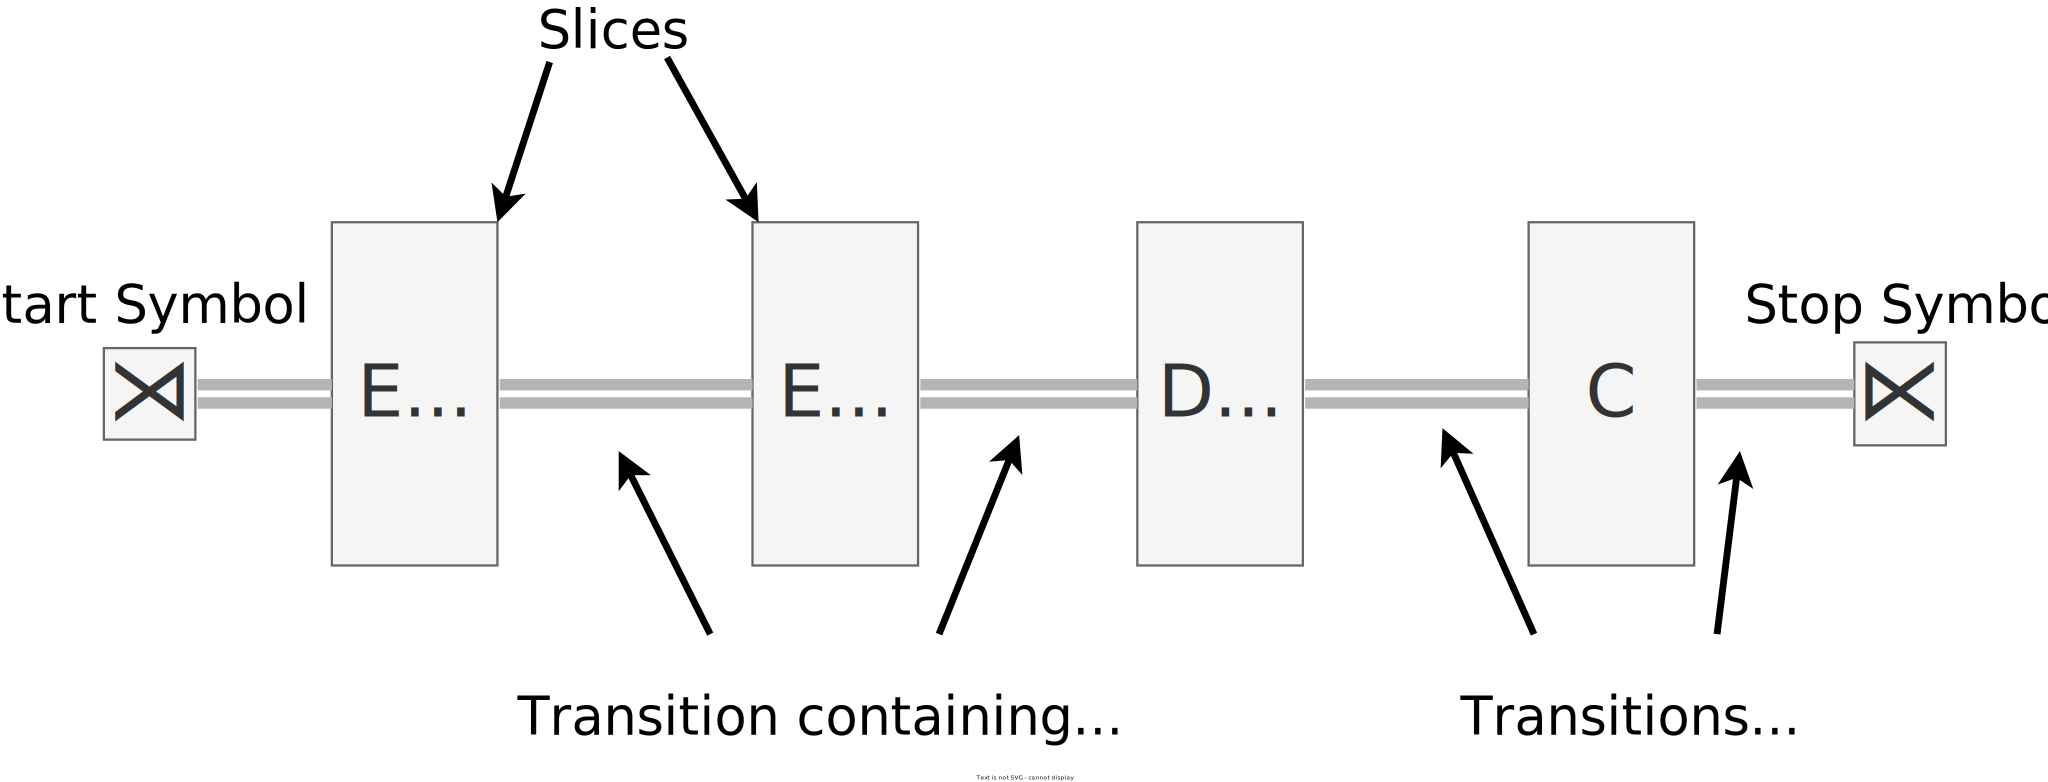
\includegraphics[width=0.9\textwidth]{figs/prep/sliceRep/sliceTransitions.pdf}
      \caption{Slices and transitions.}
      \label{fig:sliceRepTransitions}
    \end{subfigure}
    \label{fig:sliceRepresentation} 
  \end{figure}

\begin{definition}[Transition] 
  A \textit{transition} $t \in \mathcal{T}$ relates two adjacent slices, $s_l$ and $s_r$,
  with a configuration of edges $e$. 
  \begin{equation} 
    \begin{aligned} 
      t = (s_l, e, s_r)
    \end{aligned} 
    \label{eq:transition} 
  \end{equation} 
\end{definition}

  % The slices and transitions form a graph given slices as nodes and transitions as edges.
  % However, as transitions only relate sequentially adjacent slices, the outer structure is in fact a \textit{path graph}
  % and can thus be represented as a alternating list of slices and transitions.

  \begin{definition}[Path] A \texttt{path} is the data structure used to represent an alternating sequence of
    transitions and slices, where the \textit{head} of the path is accessible in constant time, defined inductively as:
    % and transitions  type of graph which can be represented as an alternating sequence of elements from two sets $A$ and $B$, defined inductively as:
      \begin{equation} 
        \begin{aligned} 
          P = t~|~t~s~P  &&&& t \in \mathcal{T},~s \in \mathcal{S}\\ 
        \end{aligned}
      \label{eq:pathGraph} 
      \end{equation} 
      \label{def:pathGraph} 
    \end{definition}

  As slices and transitions contain notes and edges respectively, slices and transitions are called \textit{outer
  structure}, and the notes and edges contained therein are called \textit{inner structure}.

\subsection{Inner Structure: Notes and Edges} 
\label{sub:Inner Structure}
The following is a restatement of the core of the proto-voice model,  as described in the original paper by Finkensiep \cite{finkensiepModelingInferringProtovoice2021}.

Internally, proto-voices are represented as a directed graph with one vertex for each note contained in a slice,
a vertex each for the beginning ($\rtimes$) and end ($\ltimes$) of the piece, and edges that indicate step-wise
connections between notes, which are contained within transitions. 
A \textit{proto-voice} is a path within this graph. The protovoice model is characterised by stepwise generative operations on notes. 
\textit{Regular edges} indicate a sequential connection between two notes, which may be \textit{elaborated} by introducing a repetition or a neighbour of either parent note, or both if the parents have the same pitch. 
The interval along a regular edge is always within a range of a step.
\textit{Passing edges} indicate connections between two notes with an interval larger than a step, introducing a new subordinate proto-voice. 
These passing edges must be filled with stepwise passing notes from either end \cite{finkensiepModelingInferringProtovoice2021}.

The generation of a piece begins with the empty piece ($\rtimes \to \ltimes$) and is defined by the recursive
application of elaboration rules.

These elaboration rules relate new child notes to one or two existing \textit{parent} notes.

\textit{Single-sided} rules attach a new repetition or neighbour note with an edge connected to a single parent note: 
\begin{equation}
  % p \implies x \to p \text{~~~~or~~~~} p \implies p \to x 
  \begin{aligned} 
    x &\implies n \to x && \text{\texttt{left-neighbor}} \\ 
    x &\implies x \to n && \text{\texttt{right-neighbor}} \\ 
    x &\implies x' \to x && \text{\texttt{repeat-before}} \\ 
    x &\implies x \to x' && \text{\texttt{repeat-after}} \\ 
  \end{aligned}
% \label{eq:singlesidedinnerop}
\end{equation}

\textit{Double-sided} rules are represented by \textit{edge replacement}. 

\begin{equation} 
  \begin{aligned}
    \rtimes \to \ltimes &\implies \rtimes \to x \to \ltimes && \text{\texttt{root-note}} \\ 
    x_1 \to x_1 &\implies x_1 \to x' \to x_2 && \text{\texttt{full-repeat}} \\
    x \to y &\implies x \to y' \to y && \text{\texttt{repeat-before'}} \\
    x \to y &\implies x \to x' \to y && \text{\texttt{repeat-after'}} \\ 
    x_1 \to x_1 &\implies x_1 \to n \to x_2 && \text{\texttt{full-neighbor}} \\
\end{aligned} 
% p_1 \to p_2 ~~~\implies~~ p_1 \to c \to p_2 \label{edge replacement}
\label{eq:doublesidedinnerop} \end{equation}

\textit{Passing} rules, finally, fill passing edges with notes from the left or right until the progression is fully stepwise.

\begin{equation} 
  \begin{aligned} 
    x \dashrightarrow y &\implies &x \to p &\dashrightarrow y && \text{\texttt{passing-left}} \\ 
    x \dashrightarrow y &\implies &x \dashrightarrow p &\to y && \text{\texttt{passing-right}} \\
    x \dashrightarrow y &\implies &x \dashrightarrow p &\to y && \text{\texttt{passing-final}} \\ 
\end{aligned}  
\end{equation}
  % Recall that the raw input is a sequence of notes with precise descriptions of where each note begins (onset) and ends (offset). 

% [Start from the sliced based formulation.]
%
% [The protovoice model is a formal generative model which represents a piece of music as a graph where each note is
% a node, and the edges between nodes represent relations between notes. ]

The inner structure provided by protovoices captures the sequential and functional organisation of notes, but does not
capture when notes are simultaneous. To model simultaneity, notes and edges are integrated into the outer structure of
slices and transitions as described in Section~\ref{sub:slicesTransitions}. 

\subsection{Generative Proto-voice Operations}
\label{sub:pvOps}

  \begin{figure}[ht] \centering 
    \begin{subfigure}[t]{.23\textwidth}
    \centering\includegraphics[keepaspectratio,width=\textwidth]{prep/outer/split} 
    \caption{\texttt{split}}
    \label{fig:splitOp} 
    \end{subfigure} 
    \begin{subfigure}[t]{.38\textwidth}
    \centering\includegraphics[keepaspectratio,width=0.91\textwidth]{prep/outer/spread} 
    \caption{\texttt{spread}}
    \label{fig:spreadOP} 
    \end{subfigure} 
    \begin{subfigure}[t]{.20\textwidth}
    \centering
    \includegraphics[keepaspectratio,width=\textwidth]{prep/outer/freeze} \caption{\texttt{freeze}}
    \label{fig:freezeOp} 
      \end{subfigure} 
    \centering 
    \captionsetup{width=.9\linewidth} 
    \caption{\small The three operations on outer structure. The original slices and transitions are shown at the top, while the generated structure is shown underneath. Figure reproduced from original paper \cite{finkensiepStructureFreePolyphony2023}}
\label{fig:outerOperations} 
\end{figure}

    The outer structure is generated through the recursive application of three production rules:

    \begin{itemize} \item A \textbf{split} replaces a parent transition $t$ by inserting a new slice $s'$ and two
      surrounding transitions $t_l$ and $t_r$. One or more inner operations can be applied to each of the edges in
      $t$, and the resulting edges can be discarded or kept to form the new edges of $t_l$ and $t_r$. 
      \begin{equation} t \to t'_l~s'~t'_r \label{eq:splitrule} \end{equation} 
      \item A \textbf{spread}
      replaces a parent slice $s$ by distributing its notes to two child slices $s'_l$ and $s'_r$. 
      This allows a vertical configuration of notes (i.e a slice) to become sequential, thereby generating implied
      harmonies such as those produced by broken chords, chords played without all the notes beginning simultaneously. These latent harmonies can also exist within a single melodic
      line, thus a single melody can be generated from an implied harmony. During a spread, passing edges can be
      introduced between any two of the child slices. 

      \begin{equation} t_l~s~t_r \to t'_l~s'_l~t'_m~s'_r~t'_r \label{eq:spreadrule} \end{equation} 
      \item A \textbf{freeze} marks a transition as terminal, preventing any further application of operations to its edges. 
  \begin{equation} t \to \underline{t} \label{eq:freezerule} \end{equation} 
\end{itemize}

\begin{figure}[ht] \centering \begin{subfigure}[t]{.5\textwidth}
  \centering\includegraphics[keepaspectratio,width=\textwidth]{prep/cadenceouterder.png} \caption{Slices and
  transitions} \label{fig:cadenceOuterDer} \end{subfigure} \begin{subfigure}[t]{.42\textwidth}
  \centering\includegraphics[keepaspectratio,width=\textwidth]{prep/cadenceinnerder.png} \caption{Notes and Edges}
  \label{fig:cadenceInnerDer} \end{subfigure} \begin{subfigure}[t]{.8\textwidth}
\centering\includegraphics[keepaspectratio,width=\textwidth]{prep/cadencederivation.png} \caption{Abstract notation}
\label{fig:cadenceDerivation} \end{subfigure}
\captionsetup{width=.9\linewidth} 
\caption{An example derivation of a short phrase.
} \label{fig:innerOuterStructure} 
\end{figure}

Figure~\ref{fig:innerOuterStructure} gives an example derivation of a short phrase. 
In Figure~\ref{fig:cadenceOuterDer}, nine outer operations have been applied to generate the surface.
The generation of the piece begins with an initial split operation (1) which comprises two elaborations of the initial
regular edge, both using the \texttt{root-note} rule, introducing child notes E and C. 
Next, a spread operation (2) distributes the notes in the parent slice to the two child slices, with the first slice inheriting both notes, and the second child slice inheriting just the C. 
This spread introduces a passing edge between E and C, shown as the dashed line in Figure~\ref{fig:cadenceInnerDer}. 
The next \texttt{split} (3) elaborates the passing edge between E and
C with the \texttt{passing-final} rule,
introduce a child passing note, D. The regular edge between the two C's is elaborated using the
\texttt{full-neighbour} rule, generating the B. The final \texttt{split} (4) introduces a \textit{repetition}, E, and
a \textit{neighbour}, B, both through double-sided regular operations. Finally, the five surface transitions are marked
as terminal (5-9), indicating the surface has been fully generated. Note that these freeze operations could've been
applied in many different permutations, with the only constraint being that no more operations are applied after a transition is frozen.

Note that the vertically aligned notes in Figure~\ref{fig:cadenceInnerDer}
correspond to the notes in the surface slices in Figure~\ref{fig:cadenceOuterDer}, and the final surface shown on the
right of Figure~\ref{fig:cadenceDerivation}. 

% subsection Inner Structure (end)
% subsection Outer Structure (end)

\section{Overview of Project Aims} % (fold) 
\label{sec:protoVoiceParser}
This project aims to address the \textbf{exponential time complexity} of the original proto-voice parser by developing
a \textbf{novel heuristic} used to guide an efficient beam search algorithm to find \textbf{excellent solutions} in
\textbf{linear time}.

There are two input dimensions in this problem. 
First is the number of notes in each slice, referred to as the size of the slice, $m$.  
The worst case is dominated by the number of possible \texttt{unsplit} reductions at a single step, which corresponds to to the number of configurations of inner operations involved. 
The number of possible inner operations is dominated in the worst case by the number of double-sided operations, $\mathcal{O}(|\textit{parents}|^2 \cdot |\textit{children}|) = \mathcal{O}(m^3)$. 
    As a \texttt{split} operation can consist of any configuration of these inner operations, the number of \texttt{split} operations is $\mathcal{O}(2^{m^3})
    = \mathcal{O}(2^m)$ where $m$ is the size of the slices involved and $c$ is a constant.
    The second input is the number of slices in the original surface, referred to as the length of the surface, $n$.
    In the worst case, the total number of complete reductions is given by $\mathcal{O}(2^{m^{n}})
    = \mathcal{O}(2^{m \cdot n})$. 
    Thus the number of possible reductions is \textbf{exponential} with respect to \textbf{two inputs}, the size of each slice $m$ and the length of the surface $n$. 

I propose and implement a novel stochastic beam search algorithm to handle these dimensions of complexity in
Section~\ref{sub:searchImpl}. In order to achieve this, a heuristic fitness function is developed that provides an approximate
score for each partial reduction. This fitness function can be decomposed into each reduction step, allowing it to be
used to score each reduction step, giving more musically meaningful reductions a greater fitness score. 
Finally, a new harmony parser is developed that adds constraints to ensure chord segments are preserved throughout the reduction.
 
% The \texttt{proto-voices haskell} repository contains an implementation of a generic greedy parser for the proto-voice
% grammar which is adapted in
% this project. This parser takes a \textit{policy} function that is used to pick a reduction option in each step. It
% finds a complete \textit{left-most} derivation for a given surface, meaning the derivation is described as a sequence of
% operations (\texttt{split}, \texttt{spread}, \texttt{freeze}) applied to the empty piece ($\rtimes \to \ltimes$) in
% order, with each operation being applied to the left-most non-terminal transition. 

% In order to adapt this parser to find a plausible chord segment reduction, 
%
% there are \textbf{three key problems} to be solved: 
%
% \begin{enumerate}
%   \item Adapting the protovoice parser to perform a \textbf{chord segment reduction} process. In its current form, the
%     parser finds a complete derivation of the surface from the empty piece. Instead, the parser needs to find a \textit{reduction}
%     consisting of a single slice per chord segment, with the notes of each slice emphasising the
%     harmony of the chord segment, while explaining away the extraneous notes through the reduction steps.
%
%   \item Judging the \textbf{relative plausibility of derivations}. The existing greedy parser provides a random choice
%     policy which randomly chooses each reduction step. Although all reductions are valid, most of them are not musically
%     meaningful. I propose and implement a heuristic to solve this problem in Section~\ref{sub:heuristicDesign}.
%
% \end{enumerate}

% [This section should actually describe the existing protovoice parser\\ 
% , introduce left-most derivations, and explain that it finds a full reduction,
% , problems with the parser are 3 fold: huge search space, how to choose derivations,
% , how to reduce while maintaining harmonic information. 
% signpost this this is he parser that is adapted for harmonic reduction.]
%
% \label{sub:protovoiceParsing} An \textit{ambiguous grammar} is a context-free grammar for
% which a string can have multiple derivations. In this case, naive parsing results in a \textit{parse forest}, a set of
% possible derivations of a particular string. In many cases, such an exhaustive parse is not possible as a result of
% a combinatorial explosion. With highly ambiguous grammars, such as those describing natural language, or the protovoice
% model, only a small subset of derivations produced by a grammar are \textit{plausible}. For a parse to be useful, it
% should yield a plausible derivation.
%
% In the case of the protovoice model, a \textit{plausible} derivation is one which is consistent with a valid musical
% \textit{interpretation}. Although this is non-trivial, derivation plausibility can be approximately represented by
% a probability distribution, analogously to probabilistic context free grammars(PCFGs). \par
% \footnote{
% [Christoph: "valid" is not enough, all PV derivations correspond to a valid interpretation. Plausibility is something
% that comes on top of that. You could just say, that plausibility can generally be characterized by a distribution P(d).
% Then you may (or may not) argue that it's useful to express this joint distribution as a series of conditionals, one per
% step. You might actually consider not doing that since the distribution you define later doesn't consist of conditionals
% but of "potentials" (arbitrary factors that are normalized in the end). The argument about finding the best derivation
% still works, you just have to say that you want to go from $p(D)$ to $\argmax_D p(D|S)$, where $p(D|S) = P(D,S)/P(S)
% = P(S|D) * P(D) / P(S)$. As before, $P(S|D)$ is just an indicator (does D generate S?) and P(S) is a constant.
%
% One thing to note here is that PCFGs are way more specific models than the general factorization in Eq. 2.21, since they
% assume that the probability of a rule application only depends on the symbol it's applied to, and not all previous steps
% $(d_0, ..., d_i-1)$.]
% }
% \begin{definition}[Reduction] A \textit{reduction} is defined as as the inverse of a generative process, and is
% synonymous with a \textit{derivation}. When parsing we \textit{reduce} a piece by applying inverses of the generative
% operations. The structure midway through a parse of a surface is called a \textit{partial reduction} of that surface.
% \end{definition}
% \par \begin{definition}[Derivation plausibility] The plausibility of a derivation is given by the product of the
%   probabilities of each of the production rules used. Given a derivation $D$ consisting of $N$ operations, its
%   plausibility is defined: \begin{equation} p(D) = \prod_{i}^N p(d_i| d_0, \dots , d_{i-1}) \end{equation}
% \end{definition}
%
% Where $d_0$ is the first step in the generative direction. Assuming we can calculate $p(D_i|S)$, we can find the most
% plausible derivation by taking the maximum likelihood estimate (MLE) of the distribution \begin{equation} \hat
% D = \argmax_{D}  p(D|S) \label{eq:mapApproach} \end{equation}
%
% This presents \textbf{two key problems} to be solved: 
% \begin{itemize} \item \textbf{Calculating} $p(d_i|d_{>i})$.
%   Production probabilities can be viewed as parameters of the model; a common approach with PCFGs is to learn these
%   parameters using machine learning. However, as the protovoice model is not context-free and the volume of data
%   required is not available an alternative method must be found. Furthermore, this would require a top down parse, which
%   is not computationally viable. \item \textbf{Combinatorial explosion}: Even if finding the maximum $P(D|S)$ could be solved analytically, the computation would be prohibited by the large branching factor.
%   % \footnote{I need a better way to represent the scale here. Perhaps I'll try to actually estimate a number}.
% \end{itemize}
%
% subsection Voices (end)
\FloatBarrier 
% \section{Search Algorithms}
% \label{sec:searchAlgos}
%
% Heuristic search algorithms are introduced in 1B \textit{Artificial Intelligence}, so it is therefore assumed the reader
% has knowledge of the heuristic search paradigm.
%
% In this project, the task of finding a reduction is framed as a search problem.
% % Parsing can be defined as a search problem wherein the goal is to find a valid derivation of the input according to
% % a grammar. 
% The search space consists of partial reductions, and begins with the original unreduced surface. The space is defined by a \textbf{directed acyclic graph} (DAG), with edges corresponding to the inverse of the generative rules. 
% An \textit{exhaustive search} strategy would theoretically allow us to find the most plausible derivation (assuming we
% can judge their plausibilities), but is computationally infeasible.
%
% \textbf{Best-first search} is a heuristic search algorithm maintains a frontier, and selects the most \textit{promising}
% node in the frontier to expand based on a heuristic evaluation function. In general, the heuristic function $h(n)$ depends on  the description of $n$, the description of the goal, information gathered by the search up to that point, and most importantly domain specific
% knowledge\cite{pearlHeuristicsIntelligentSearch1984}. 
% Best-first suffers from memory problems if the frontier becomes very large.
%
% \textbf{Beam search} is an optimisation of best-first search that serves to reduce its memory requirements by expanding
% all of the nodes in the frontier simultaneously and
% updating the frontier to consist of only the $\beta$ best of the expanded states, where $\beta$ is the \textit{beam
% width}. Beam search is greedy algorithm, so it does not necessarily produce the optimal solution (according to the
% heuristic), but trades optimality for improved complexity. Beam search suffers from lack of diversity as the beam tends to get dominated by expansions of a low cost state, causing the search to get stuck in local optima.
%
% \textbf{Stochastic beam search} is a further optimisation of beam search 
%
% of best-first search that serves to reduce its memory requirements by only storing a limited number of best states as
% candidates to expand, dependent on the \textit{beam width}. 

% Heuristic search algorithms are a subset of search algorithms used to find a sequence of actions from an initial state
% that results in a goal state.  The problem is defined as follows: \begin{itemize} \item We have an \textit{initial
% state} $s_0$ where $s_0 \in S$, the set of possible states \item We have set of \textit{actions} $A$, modelled by the
% function $action: A\times S \to S$ \item We have \textit{goal test}, modelled by the function $goal: S \to \{true,
% false\}$ \item There is a \textit{cost} associated with every path, modelled by $cost: A \times S \to \mathbb{R}$
% \item Finally, we have a function \textit{expand} is a \textit{cost} associated with every path, modelled by $cost:
% A \times S \to \mathbb{R}$ \item We wish to find the minimum cost path from the initial state $s_0$ to a goal state.
% % \item We have an initial state $s_o \in S$, which is the empty reduction, corresponding to the unreduced surface of
% the piece. The score is represented as a sequence of slices grouping notes that sound simultaneously. We are also
% given the segmentation of the original chord labels that we wish to retrieve. % \item We have a set of actions, $A$
% modelled by a function $action: A \times S \to S$. These actions correspond to a single reduction step.
% %   \begin{itemize} %     \item The reduction steps are the inverses of the operations defined by the generative
% proto-voice model. %   \end{itemize} % \item Finally we have a goal test, $goal: S \to \{true,false\}$ which is true
% iff the partial reduction $s$ has exactly one slice per segment of the input. %   \begin {itemize} % \item This means
% the partial reduction $s$ contains a sequence of slices which start and end positions corresponding to the
% segmentation of the piece. %   \end {itemize} % \item At the first stage, this will be implemented using a random
% graph search algorithm, picking each action randomly, according to precomputed distributions. % \item The state space
% $S$ is the set of all possible partial reductions of a piece along with each reduction step that has been done so far.
% % \item We have an initial state $s_o \in S$, which is the empty reduction, corresponding to the unreduced surface of
% the piece. The score is represented as a sequence of slices grouping notes that sound simultaneously. We are also
% given the segmentation of the original chord labels that we wish to retrieve. % \item We have a set of actions, $A$
% modelled by a function $action: A \times S \to S$. These actions correspond to a single reduction step.
% %   \begin{itemize} %     \item The reduction steps are the inverses of the operations defined by the generative
% proto-voice model. %   \end{itemize} % \item Finally we have a goal test, $goal: S \to \{true,false\}$ which is true
% iff the partial reduction $s$ has exactly one slice per segment of the input. %   \begin {itemize} % \item This means
% the partial reduction $s$ contains a sequence of slices which start and end positions corresponding to the
% segmentation of the piece. %   \end {itemize} % \item At the first stage, this will be implemented using a random
% graph search algorithm, picking each action randomly, according to precomputed distributions. \end{itemize}
%
% subsection protovoiceParsing (end)
    % the sum over all values of $Z$ can be avoided by finding $\hat{Z} = \argmax_Z
    % P(Z|X) $, the most likely value of $Z$ given $X$, using MLE or MAP estimation.
    % The prior $P(Z|X)$ is updated as follows as follows: \[P(Z|X) = \begin{cases} 1 &\text{if } Z=\hat{Z} \\
    % 0 &\text{otherwise}\end{cases}\]
    % This results in an approximation of $P(Y|X)$:


%       \section{Overview of Approach}
%       \label{sec:overviewApproach}
%       [Relate this directly to the actual project]
%       [Cut the bullshit]
%       [This section needs to be a huge flex]
%       % \textbf{Probabilistic inference} is a statistical inference paradigm in which Bayes' theorem is used to update the
%       % probability for a hypothesis in light of available evidence. 
%
%       \textbf{Probabilistic inference} is a statistical inference paradigm which reduces to representing the \textit{joint
%       distribution} of all the random variables in a system, such that we can compute any probability of interest in that
%       system. This allows us to \textit{infer} information about \textit{latent}(hidden) variables based on
%       observations. Let $X$ and $Z$ denote the observed and latent(unobserved) variables respectively, and
%       let $Y$ denote the random variable to be inferred. By formulating a model of the \textit{joint distribution}
%       $P(X,Y,Z)$, the most probable value of $Y$ can be inferred from the observations $X$ by solving $\argmax_Y P(Y|X)$. 
%
%       \footnote{[Christoph: This is only one particular type of inference in which you determine the most plausible
%       value of Y, to be precise. You could also infer the full posterior distribution over Y, for example.]}
%
%       % \textbf{Modelling} is the process of approximating a joint distribution through abstract representations and
%       % relationships.
%       \subsection{Tools of Probabilistic Inference}
%       [In this section, instead of explaining probability, just actually explain the approach taken broadly, while
%       defining terms when needed. ]
%
%       % We first consider how we would compute the best hypothesis for $Y$ given the evidence $X$, ignoring the latent
%       % variables $Z$. In order to infer information about the value of $Y$ given the joint distribution $P(X,Y)$ and the
%       % observation $X$, we consider the \textit{conditional} probability distribution, $P(Y|X)$. 
%
%       \begin{definition}[Marginalisation] \begin{equation} P(A) = \sum\limits_B P(A|B)~P(B) \label{eq:marginalisation}
%       \end{equation} \end{definition}
%
%
%       \begin{definition}[Chain Rule of Probability] \begin{equation} P(A,B) = P(A|B)~P(B) \label{eq:chainRule}
%       \end{equation} \end{definition}
%
%       There are broadly two methods used to find the most probable value of $Y$: 
%       \begin{itemize} \item  The \textbf{maximum
%         a posteriori estimate}(MAP) maximises the \textit{conditional probability} of $Y$ given the observations, given by
%         the posterior distribution, $P(Y|X)$. 
%         % This requires us to know the \textit{prior} $P(Y)$, the distribution of the hypothesis, beforehand. The
%         % prior can be learned from labeled data. 
%         \begin{equation} 
%           \begin{aligned} \hat{Y} &= \argmax_Y P(Y|X) \\ 
%           % &= \argmax_Y P(X|Y)P(Y) 
%           \footnote{[Christoph: This is a non-trivial step that uses the rule of Bayes: the crucial point is that p(X) is
%       a constant, but that term isn't shown here.]}
%       \end{aligned} \label{eq:map} 
%         \end{equation} 
%         \item  The \textbf{maximum likelihood estimate}(MLE)
%         maximises the likelihood of the observations given the hypothesis, given by the likelihood, $P(X|Y)$. 
%         % This method allows us to capture \textit{uncertainty} in the prediction, given by $P(X|\hat{Y})$.
%         \begin{equation} \hat{Y} = \argmax_Y P(X|Y) \label{eq:mle} \end{equation} 
%       \end{itemize}
%   %
%       % \begin{definition}[Factoring] \begin{equation} P(A,B) = P(B|A)~P(A) \label{eq:bayesRule} \end{equation}
%       % \end{definition}
%   %
%
%       % \subsection{Introducing Latent variables} 
%       To incorporate the latent variables $Z$, \textit{marginalisation} and the \textit{chain rule of probability} are used to show that: \begin{equation} \begin{aligned}
%       P(Y|X) &= \sum\limits_Z P(Y,Z|X) \\ &= \sum\limits_Z P(Y|X,Z)~P(Z|X) \end{aligned} \label{eq:} \end{equation}
%
%       Given an abstract model $P(Z,X)$, the marginal distribution can be approximated by the distribution where $Z$
%       is assumed to have the MAP value $\hat{Z}$, resulting in:
%
%         \begin{equation} 
%           \begin{aligned}
%             P(Y|X) &= \sum\limits_Z P(Y,Z|X) \\
%                    &\approx P(Y|X,\hat{Z})  \\
%             
%           \end{aligned}
%       \label{eq:inferenceTrick} 
%         \end{equation}
%
%
%       % \textbf{Probabilistic programming} is a programming paradigm that makes use of model definitions and statistical
%       % inference algorithms to compute the conditional distribution of inputs that could have given rise to an observed
%       % output. 
%
%       % In the context of ACE, the \textbf{input} is the underlying sequence of chord labels $L_0, L_1,\dots L_n$, and the
%       % score is the \textbf{observed output} $S$. 
%  % Implementation
% % The result of this project is the ProtoVoice Harmony Model, a     
%       Recall that ACE can be solved by finding the most likely sequence of labels for the given surface, described by the equation: 
%
%       \begin{equation} \hat L = \argmax_L P\left(L|S\right) \label{eq:aceProbSol} \end{equation}
%
%       The difficulty arises from the complexity and prohibitively large number of the \textbf{latent variables} $\bm{
%       \phi }$; in reality, we need to maximise $\sum\limits_{\bm{\phi}}P(L|S,\bm{ \phi })~P(\bm{\phi}|S)$.
%
%       \begin{equation} \hat L = \argmax_L \sum\limits_{\bm{\phi}} P(L | S,\bm{\phi})~P(\bm{\phi}|S)
%       \label{eq:aceProbSolLatent} \end{equation}
%
%       The set of latent variables $\bm{\phi}$ is \textbf{practically infinite}. These include the author's compositional
%       conception, their musical conception, cognitive phenomena experienced by listeners, shared experience distilled
%       into music theory, musical trends/culture and notational conventions. This distribution is unknown and far to
%       complex to be described fully, but $\hat{L}$ can be approximated using models that encode domain specific knowledge about both the music generation and labelling processes, combined with efficient inference algorithms. 
%
% %       \subsubsection{Approximating Conditional Likelihood with MLE}
% %
% %       Now consider the set of latent RVs $\bm{\phi}$ as the union of two \textit{disjoint sets}, $\bm{\phi'}$ and
% %       $\bm{\phi''}$, where $\bm{\phi'}$ is the subset of $\bm{\phi}$ which we can \textit{infer} given $L$ and $S$, and
% %       $\bm{\phi''} = \bm{\phi} \setminus \bm{\phi}'$. Assuming $P(\bm{\phi'} | L)$ and $P(\bm{\phi''} | L)$ are
% %       independent, it follows:
% %
% %       \begin{equation} \begin{aligned} P(L|S) &= \sum\limits_{\bm{\phi'}}\sum\limits_{\bm{\phi''}} P(L
% %       | S,\bm{\phi'},\bm{ \phi'' })~P(\bm{ \phi' }, \bm{ \phi'' } |S) \\ &=
% %     \sum\limits_{\bm{\phi'}}\sum\limits_{\bm{\phi''}} P(L | S,\bm{\phi'},\bm{\phi''})~P(\bm{\phi'} | S)~P(\bm{\phi''}
% %   |S) \end{aligned}
% %   % \hat L = \argmax_L \sum\limits_{\phi} P(S | L,\phi)~P(\phi|L)
% % \label{eq:aceProbSolLatent} \end{equation}
% %
% % The uniform distribution is used to model $P(\phi''|S)$ as we have no prior knowledge of those latent variables. Using
% % the technique described in Equation~\ref{eq:inferenceTrick}, we find $\hat{\phi'}$, thus giving: 
% %
% % \begin{equation} \begin{aligned} \hat L \approx \argmax_L P(L | S, \hat{\phi'}) \end{aligned}
% % % \hat L = \argmax_L \sum\limits_{\phi} P(S | L,\phi)~P(\phi|L)
% % \label{eq:aceProbSolLatent} \end{equation}
% %
% %
% %
% %
% %
% %
% %

%
%
% We achieve this by only considering the latent variables $\phi'$ that we can reasonably \textit{infer}, discarding the
% rest of $\phi$ by assuming $P(\phi|\phi')$ is a uniform distribution. In this project, we use the protovoice model to
% infer the latent structure of the surface $\hat{D}$, and thus calculate $p(S|L,\hat{D})$.

\section{Requirements Analysis}
\label{sec:requirementsAnalysis}
% \subsubsection{Success Criteria}
The Success Criteria are given in the \nameref{chap:proposal}. During the preparation phase, the Success Criteria were
refined in light of increased clarity from reading the literature related to the project. Concretely, the final Success
Criterion given in the Proposal describing the development of heuristic search algorithms has been divided into two
criteria, developing the heuristic, and developing the search algorithms.

This project will be deemed a success given it achieves: 
\begin{itemize} 
  \item A harmony module that can use a reduced surface to infer chord labels, and quantitatively evaluate its accuracy against the ground truth annotations. 
  \item A heuristic fitness function that can be used to judge the relative plausibility of derivations. 
  \item An implementation of a new parser for the protovoice model which finds possible reductions of a musical surface. 
  \item Extension: One or more search algorithms that make use of the developed heuristic to inform the search, dealing with the two dimensions of exponential complexity. 
\end{itemize} 

\begin{table}[ht] \caption{Project Deliverables} 
  \vspace{\baselineskip} 
  \label{tab:deliverables} 
  \centering
  \begin{tabularx}{0.9\textwidth}{cXcc} 
    {\large \textbf{ID}} & \large \textbf{Deliverable} & \large \textbf{Priority} & \large \textbf{Risk} \\ 
    \toprule 
    \texttt{core1} & Harmony Model & High & Low \\ 
    \texttt{core2} & End to End Pipeline & High & Medium \\ 
    \texttt{core3} & Proto-voice Harmony Parser & High & High \\ 
    \texttt{base1} & Templating Algorithm & High & Low \\ 
    \texttt{algo1} & Random Parse & High & Low \\ 
    \texttt{ext1} & Heuristic Design & Medium & High \\
    \texttt{ext2} & Heuristic Search & Low & Very High \\
\end{tabularx} \end{table}

\subsubsection{Risk Analysis}
\label{sub:riskAnalysis}

This project has a high general risk factor as it involves a \textbf{novel} approach to inferring harmony. 
Table~\ref{tab:deliverables} shows a list of project
deliverables with associated priorities and risk, denoted qualitatively. 
The task with the greatest risk attached is designing and implementing the protovoice harmony parser, as this requires understanding and building on a complex existing codebase, and my proposed adaptation of the proto-voice parser has not been implemented before. 
Designing a bottom-up heuristic has a high risk factor as this is also a novel task, requiring creativity, research and iterative development. 
The baseline inference deliverable implements a standard chord templating method used commonly for ACE \cite{pardoAlgorithmsChordalAnalysis2002}, posing minimal risk. 
Finally, the design and optimisation of efficient search algorithms is also a substantial task, which runs the risk of sinking a practically infinite amount of time.

In order to mitigate the risks posed by this project, the heuristic design and heuristic search tasks were set as
extensions, so that only one high risk task was in the core part of this project.

\section{Software Engineering Techniques}
\label{sec:softwareEnginerring}

\subsection{Development model}
\label{sub:devModel}

Based on the risk analysis (Table~\ref{tab:deliverables}), a plan was created describing which modules to implement in
which order, with a list of milestones on a 2 week basis. Notion was used to maintain a list of core tasks and
corresponding subtasks with associated priorities, facilitating the selection of the next tasks to work on. The
development strategy chosen drew from the Agile methodology, involving two-week long sprints with regular re-evaluations
of the plan informed by experimental data and testing. GitHub's continuous integration features were used to run a test
suite on the repository after every commit.  

\subsection{Languages, libraries and tools}
\label{sub:languagesLibrariesTools}

    \begin{table}[ht!] \caption{Languages, libraries and tools} \label{tab:languages} \centering \footnotesize
      \renewcommand{\arraystretch}{1.3} \begin{tabularx}{\textwidth}{p{4em}X X p{4em}} {\normalsize \textbf{Tool}}
      & {\normalsize \textbf{Purpose}} & {\normalsize\textbf{Justification}} & {\normalsize \textbf{License}} \\
        \toprule \textit{Languages} &&&\\ Haskell & Main language used for the core, baseline and extension
        implementations & Protovoice model implementation is in Haskell. Functional and amenable to parser development.
                        & GHCL \\

        Python & Secondary language for experiments and analysis & Powerful library ecosystem for running experiments
        and creating plots & PSFL \\

        \midrule \textit{Libraries} &&&\\ Musicology & Haskell Library with data-types for pitches & Contains a robust
        implementation of spelled pitch classes, which would be tedious to reimplement. & BSD-3.0 \\ Timeit & Lighweight
        wrapper to show the used CPU time of a monadic computation & This is used to measure the runtime of the algorithms
        as part of analysis & BSD-3.0 \\ Dimcat & Python library: DIgital Musicology Corpus Analysis Toolkit & This
        library was written to work with the datasets used in this project & GPL-3.0 \\ Numpy & Python library used for
        preprocessing and analysis & Powerful standard library that is used in conjunction with Seaborn to run analysis
        and visualise data & BSD-3.0 \\ Pandas & Python library for preprocessing and analysis & This is a standard
        library for data manipulation and processing & BSD-3.0 \\ Seaborn & Python data visualisation library used for
        analysis & Creates high quality graphs and charts & BSD-3.0 \\ \midrule

        \textit{Tools} &&&\\ Docker & Containerised software service used to run repeatable experiments
                       & Protects code from breaking changes and allows code to be executed on
        different devices without manually installing dependencies & Free/Paid \\ Git & Version Control, Continuous Integration & Provides natural backups and
        allows for reverts to previous commits if necessary & GPL-3.0 \\ GitHub & Hosting source code & Free, reliable
        hosting & GPL-3.0 \\ GHC & Compiling and profiling. & This is the standard Haskell compiler. & BSD-3.0 \\ Stack
                & Haskell building and testing  & Creates reliable builds, and includes a powerful testing framework.
                & BSD-3.0 \\ Undotree & Vim Plugin: stores all past actions as a tree & Solves the problem of linear
        undo history being lost. Protects code between commits. & BSD-3.0 \\ MuseScore & Music notation software & The
        raw inputs are in the MusicXML format, which is used by MuseScore 3 & GPL-3.0 \\ PAT & Protovoice Annotation
        Tool, Used to view protovoice derivations on a web browser & The protovoice derivations are huge and very
      complex, so it's vital to have a viewing tool for use in analysis and iterative development & GPL-3.0 \\
    \end{tabularx} 
  \end{table}

    Table~\ref{tab:languages} shows a justified list of the key languages, libraries and tools used in the project. The
    licensing agreements for all the tools used in the project were determined and analysed. For the most part, these
    are all permissive licenses, guaranteeing freedom to use, modify and redistribute as well as permitting proprietary
    derivative works. 

    \subsection{Hardware, version control and backup} 
    \label{sub:hardware}
    The code was developed using Vim for Haskell and Visual Studio
    Code for Python notebook development, on my personal laptop (16' MacBook Pro 2022, M1 Max, 32GB). Algorithms
    were first run on my laptop, then later run on a server provided by the EPFL Digital Cognitive Musicology Lab (Dell PowerEdge R740XD Server, 2x Xeon Gold
    625R, 768GB), using Jupyter notebooks to conduct the evaluation. I used GitHub for all my notes, development and
    dissertation writing. Finally, this dissertation was written in Vim with VimTeX.

%%%%%%%%%%%%%%%%%%%%%%%%%%%%%%%%%%%%%%%%%%%%%%%%%%%%%%%%%%%%%%%%%%%%%
    % Implementation
%%%%%%%%%%%%%%%%%%%%%%%%%%%%%%%%%%%%%%%%%%%%%%%%%%%%%%%%%%%%%%%%%%%%%

    \chapter{Implementation}
    \label{chap:implementation}
    This chapter provides a high-level overview of the project structure (Section~\ref{sec:repoOverview}),
    followed by a detailed description of the key components of the implementation. 
    First, the design and implementation of the heuristic fitness function are presented and justified
    (Section~\ref{sub:heuristicDesign}). 
    Next, the implementation details of the harmony module is discussed, including the inferences used in
    the heuristic function (Section~\ref{sec:harmonyModel}). 
    This is followed by an exposition of the novel proto-voice harmony parser
    (Section~\ref{sec:protovoiceHarmonyParser}), followed by discussion of the core algorithms implemented (Section~\ref{sec:baselineAlgorithms}), 
    including an implementation of the template matching algorithm \cite{pardoAlgorithmsChordalAnalysis2002} as
    a standard ACE baseline. 
    Then, a description of the heuristic search algorithms developed is given (Section~\ref{sub:searchImpl}). 
    Finally, the test strategies used evaluate the effectiveness of the proposed algorithms are outlined (Section~\ref{sec:testing}).

    \begin{figure}[ht] 
    \centering 
    \includegraphics[width=\textwidth]{figs/impl/blockDiag/DissBlockDiagram.png} 
    \caption{Diagram of project components} 
    \label{fig:blockDiagram} 
    \end{figure}

    \section{Repository Overview:}
    \label{sec:repoOverview}

    \begin{table}[ht!]
      \DTsetlength{0em}{1.3em}{0em}{0.7pt}{3pt}       
      \setlength{\DTbaselineskip}{15pt}  %minimum size for \normalsize
      \renewcommand{\DTstyle}{\ttfamily}
      % \centering
      \caption{Repository Overview}
      \vspace{\baselineskip}
      \label{jeff}
      \begin{tabularx}{\textwidth}{l X c}
        File/Folder & Description & LOC \\
        \toprule
        \toprule
      \begin{minipage}[t]{5.7cm}
        \dirtree{%
        .1 protovoices-haskell/.
        .2 src/.
        .3 HarmonyParser.hs \vspace{\DTbaselineskip}.
        .3 Harmony.hs.
        .3 Harmony/.
        .4 ChordLabel.
        .4 Profiles \vspace{\DTbaselineskip}.
        .3 Algorithm.hs.
        .3 Algorithm/. 
        .4 ~TemplateMatching.hs,~RandomSample.hs,~InformedReduction.hs\vspace{0.5\DTbaselineskip}.
        .4 RandomParse.hs \vspace{\DTbaselineskip}.
        .4 HeuristicSearch/.
        .5 BestFirst.hs,~Beam.hs,~StochasticBeam.hs \vspace{\DTbaselineskip}.
        .3 Heuristics.hs \vspace{\DTbaselineskip}.
        .3 FileHandling.hs.
        .3 Probability.hs \vspace{\DTbaselineskip}.
        .3 \textcolor{blue}{Common.hs}.
        .3 \textcolor{blue}{GreedyParser.hs}.
        .3 \textcolor{blue}{PVGrammar.hs,~PVGrammar/}.
        .3 \textcolor{blue}{Display.hs}\vspace{\DTbaselineskip}.
        .2 scripts/.
        .3 preprocess.py.
        .3 experiments.ipynb.
        .3 analysis.ipynb.
        .2 data/.
        .3 inputs/.
        .3 outputs/.
        .2 app/.
        .3 MainFullParse.hs\vspace{\DTbaselineskip}. 
        .2 tests/.
        }
      \end{minipage} &
      \begin{minipage}[t]{8cm}
    Root directory
    \vspace{1.2\DTbaselineskip}\\
    Harmony Parser (Section~\ref{sec:protovoiceHarmonyParser})
    \vspace{1.2\DTbaselineskip}\\
    Harmony Model (Section~\ref{sec:harmonyModel})
    \vspace{4\DTbaselineskip}\\
    Core Algorithms (Section~\ref{sec:baselineAlgorithms}) 
    \vspace{2.6\DTbaselineskip}\\
    Core Algorithm (Section~\ref{sec:baselineAlgorithms}) 
    \vspace{1.1\DTbaselineskip}\\
    Extension Algorithms (Section~\ref{sub:searchImpl}) 
    \vspace{2.9\DTbaselineskip}\\
    Heuristic Implementation (Section~\ref{sec:extensionImplementation}) 
    \vspace{1.2\DTbaselineskip}\\
    Utilities
    \vspace{1.9\DTbaselineskip}\\
    Existing code
    \vspace{4\DTbaselineskip}\\
    Experiment Pipeline (Section~\ref{sec:testing})
    \vspace{9\DTbaselineskip}\\
    Unit and Integration Tests (Section~\ref{sec:testing})
    % Unit Tests (Section x)

      \end{minipage} & 
      \begin{minipage}[t]{0.5cm}
        2272
        \vspace{0.1\DTbaselineskip}\\
        470\\
        \vspace{\DTbaselineskip}
        121\\
        \vspace{\DTbaselineskip}
        383\\
        \vspace{1.8\DTbaselineskip}
        188\\
        \vspace{3.7\DTbaselineskip}
        431\\
        \vspace{3\DTbaselineskip}
        115\\
        \vspace{2.5\DTbaselineskip}
        611\\
      \end{minipage}
    \end{tabularx}
    \end{table}

    \FloatBarrier
    \subsubsection{Repository Justification}

    The repository has broadly been split into five main modules, as illustrated in Figure~\ref{fig:blockDiagram}.
    Everything shown has been written during this project except for the files shown in blue.
    \begin{itemize} 
      \item Firstly, the \texttt{HarmonyParser.hs} contains the first core contribution, an adaptation of the greedy
        parser (shown in blue) which integrates the protovoice model with the chord segment reduction process.
      \item Next, the \texttt{Harmony} module contains functions and data-types for dealing with chord labels, and
        profiles, as well as performing probabilistic inference. 
      \item The \texttt{Algorithm} module provides a generic framework to run chord segment reduction algorithms. This
        module contains implementations of all the core algorithms, including Pardo and Birmingham's template maching
        algorithm \cite{pardoAlgorithmsChordalAnalysis2002}. Within this, the \texttt{HeuristicSearch/..} algorithms are
        those that make use of the heuristic fitness function.
      \item \texttt{Heuristics.hs} contains the novel heuristic fitness function developed. 
      \item The \texttt{experiments/} folder contains all the python code that is used for this project. Experiments
        were conducted by running the Haskell executable parameterised by the input piece and algorithm to use, and
        results are stored using \texttt{Json}. The experiments consist of three stages, as described by the three main files: \texttt{preprocess.py}, \texttt{experiments.py} and \texttt{analysis.py}. 
        Splitting these stages up prevents wasteful computation, as all the pre-processing can be done just once, while experiments are run on the processed data iteratively alongside algorithm development. 
      \item Finally, the \texttt{test/} folder contains unit tests for all of the Haskell modules, using the
        \texttt{Spec} testing framework which is used in Continuous Integration. 
    \end{itemize}


    %
    % The result of this project is the \textbf{ProtoVoice Harmony Model}, a \textbf{novel} inference system that utilises the
    % protovoice model to infer harmony from free polyphony.
    %
    % \begin{figure}[ht] \centering \includegraphics[width=\textwidth]{intro/inferenceOverview} \caption{Overview of the
    % inference process.} \label{fig:inferenceOverview} \end{figure}
    %
    % The PVHM is described by the following equation: \begin{equation} \label{eq:pvhmSuccinct} \begin{aligned} \hat{L} &=
    % \argmax_L \left( P(S|L,\hat{\mathcal{R}(S')},\hat{D})\cdot P(L)\right) \\ \end{aligned} \\ \end{equation} Where $\hat{D}$ denotes
    % the inferred \textit{protovoice derivation} of the score $S$, obtained using a modified beam search algorithm to
    % parse $S$, guided by a heuristic $\mathcal{H_0}$.  $\hat{S}$ is the associated reduction of the surface, given by
    % $top(\hat{D})$. 
    %
    % \text{where $\hat{D}$ is a \textit{protovoice derivation}} \\ \text{and:}\\ \hat{S'} = top(\hat{D})
    %
    % In the context of a protovoice derivation, the $surface$ refers to the input, the original score to be parsed, and
    % the result of the parse is the $top$ of the derivation. The core of the PVHM is finding the most likely reduction
    % $\mathcal{R}(S)$ of the surface $S$ by inferring the most likely protovoice structure $\hat{D}$. The baseline
    % algorithm achieves through a random search through the space of valid partial derivations. The extension algorithms
    % use an informed heuristic $H_0$ to guess $P(D|S)$ in order to guide the search, and explore the trade-offs between
    % exploration and exploitation with different search algorithms. Given the inferred derivation, the corresponding
    % reduced surface is extracted with $top:\mathbf{D} \to \mathcal{R}(S)$. Finally, the reduced surface $\mathcal{R}(S)$ is
    % used to solve $\hat{L} = \argmax_L P(L|S, \mathcal{R}(S)) \cdot P(L)$, finding the most likely sequence of chord
    % labels $\hat{L}$. 
    %

    % \subsubsection{Development plan} This system is modular by design, leading to a natural progression of complexity
    % throughout the implementation; the baseline models provide a subset of the functionality required for the full
    % system. For example, the harmony model is a prerequisite for the first baseline, but is also used in all subsequent
    % models. \footnote{This could be complemented by a diagram showing the progression}
    %
    % \begin{itemize} \item The Baseline Reduction computes a simplified $\mathcal{R}(S)$ using random sampling. \item The
    %   Random Search uses $\mathcal{R}(S) = top (D_0)$, where $D_0$ is the derivation found by randomly choosing each
    %   parse operation. \item The first extension involves developing an informed heuristic $\mathcal{H}_0$ to evaluate
    %   the plausibility of different parse states. \item The
    %   Greedy Search uses heuristic $\mathcal{H}_0$ to approximate $\argmax_D P(D|S)$. \item Finally, the Heuristic Search uses
    %   $\mathcal{H}_0$ to implement a more advanced stochastic search algorithm. 
    %   % by the beam width $\beta$ \item The Dual Beam Search
    %   % implements a custom search algorithm using $\mathcal{H}_0$, parameterised by $\alpha$ and $\beta$, which control
    %   % operation dependent beam widths.  
    % \end{itemize}

      % \begin{equation} P(S|L) = \sum\limits_{D,S'} P(S|D)~P(D|S')~P(S'|L) \label{eq:inferencePVEQ} \end{equation} The
      % repository for this project is a fork of an existing repository that contains useful data-types and functions
      % for working with the protovoice model \cite{finkensiepModelingInferringProtovoice2021}. Uses these allows for
      % interoperability with other projects involving the model.

      % \section{Core Implementation}


      % \begin{itemize} \item First we use the \textit{protovoice model} to \textit{reduce} a musical surface,
      % simplifying the score by removing redundant notes from the surface, using domain specific knowledge to infer the
      % most likely latent structure, $\hat{D}$, which is in turn used to infer the most likely reduced surface, $S'$.
      % % \footnote{We are relying on the assumption that this structure is somehow shared between the processes of
      % composition, listening, and analysis. This is a fair assumption to make given they are all considering the same
      % thing.}. \item Subsequently, using a \textit{harmony model} $P(S'|L)$ we find the conditional likelihood of the
      % \textit{reduced} surface $S'$ given a hypothesised sequence of labels, $L$.
      %   \item Finally, we choose the sequence of labels $\hat{L}$ that \textit{maximises the likelihood} of the
      %   reduced score. \end{itemize}
%
      % We find a \textbf{reduction} of the original surface $S$, denoted $\hat{S'} = top(\argmax_D P(D|S))$
%
      % The approach taken in the PVHM is as follows:
%
%
%
      % The method I will use to infer harmony using the protovoice model is to find a plausible \textit{reduced
      % surface} $S'$ which has one slice per chord label, having explicitly explained away non chord-tones
      % (ornamentations) through protovoice edges. Given this, the chord labels can be inferred using a model of
      % harmony.

    % This section first motivates  the implementation of the efficient fitness function, including a number of optimisations
    % (Section~\ref{sub:heuristicImplementation}), then justifies the design of the fitness function (Section~\ref{sub:heuristicDesign}).
    \newpage
    \section{Proto-voice Fitness Function}
    \label{sec:extensionImplementation}

    To address the \textbf{exponential time} complexity of the naive parser and enable the efficient identification of musically
    meaningful proto-voice derivations, I propose a \textbf{novel fitness function} that evaluates a plausibility score
    for each
    derivation. The fitness function decomposes into a score for each reduction step and is used to guide the
    efficient heuristic search algorithm designed in Section~\ref{sec:evalExtension}, allowing \textbf{excellent
    solutions} to be found in \textbf{linear time}.


    \subsection{Motivation of Fitness Function}
    \label{sub:heuristicDesign}


    The proto-voice fitness function is motivated by defining a probability distribution for proto-voice
    derivations, $P(\vec{d})$, factored into each derivation step. 
    Given a derivation $\vec{d} = d_0 \dots d_N$ define: 

    \begin{equation}
      P(\vec{d}) = \frac{1}{Z} \prod_i \phi (d_i)
      \label{eq:}
    \end{equation}

    Where $Z$ is the normalisation constant, and $\phi$ is a heuristic function that defines a relative probability for
    each reduction step, consisting of two factors corresponding to the generative proto-voice operations. 

    \begin{equation}
      \phi(d_i) = \phi_{\texttt{parents}}(d_i) \cdot \phi_{\texttt{children}}(d_i)
      % \phi_{\texttt{harmony}}(d_i)^{\zeta}
      \label{eq:}
    \end{equation}

    The \texttt{parents} factor evaluates the relative plausibility of the parent notes chosen to be elaborated in the
    operation, and the \texttt{children} factor evaluates the relative plausibility of the child notes introduced from
    those parents. 
    % Finally, the \texttt{harmony} factor is used to encourage derivations that result in more probable harmonic structures.
    
    Conditioning this distribution on the input sequence $S$, it follows from Bayes' Rule: 

    \begin{equation}
      \begin{gathered}
      P(\vec{d}|S) = \frac{P(S|\vec{d})\cdot P(\vec{d})}{P(S)} = P(S|\vec{d})\frac{1}{P(S)} \frac{1}{Z} \prod_i \phi(d_i) \\
      \text{where } P(S|\vec{d}) = 
        \begin{cases} 
          1 & \text{if } \vec{d} \text{ produces } $S$ \\
          0 & \text{otherwise}
        \end{cases}
      \end{gathered}
      \label{eq:}
    \end{equation}
    
    It is guaranteed (see Section~\ref{sec:testing}) that any derivation $\vec{d}$ found by the proto-voice harmony
    parser produces $S$, so $P(S|\vec{d})$ is always $1$. Computing the normalisation constant, $\frac{1}{P(S)\cdot
    Z}$, is intractable, but for the purpose of maximisation it can be ignored. It therefore suffices to compute
    $P(\vec{d}) = \frac{1}{Z} \prod_i \phi (d_i)$. 

    \subsubsection{Justification}

    It is informative to consider how a true generative probability distribution for proto-voice derivations would be
    structured. 
    The probability of a derivation $\vec{d}$ in the generative direction is naturally factored into each derivation step as
    follows:
    \begin{equation} 
      p(\vec{d}) = \prod_{i}^N p(d_i| d_0, \dots , d_{i-1}) 
    \end{equation}
    Where $d_0$ is the first generation step. A generative model would factorise this expression into
    conditionals that correspond to the generation steps, thus providing a guess of the distribution
    $p(\vec{d})$. Instead, the fitness function approximates this overall distribution based on local
    plausibility properties, corresponding to $\phi$. This approximation allows the fitness function to remain
    computationally tractable while capturing essential aspects of the true generative distribution.

    \subsection{Implementation of Fitness Function}
    \label{sub:heuristicImplementation}

    In this section, Algorithm~\ref{code:pvff} is walked through step-by-step, discussing any relevant implementation details and justifying
    design decisions where appropriate. 
    At a high level, the fitness function provides a score for partial derivations by partial application of each derivation step during the search. 

    \begin{algorithm}
    \caption{Proto-voice Fitness Function}
    \begin{algorithmic}[1]
      \Require {derivation, \texttt{surface}}
      \Ensure 
      \State Initialise fitness score $F \gets 1$             
      \For{each reduction step $d_i$ in derivation}
          \If{$d_i$ is a freeze operation}
              \State $P(d_i) \gets 1$
          \ElsIf{$d_i$ is a split or spread operation}
            \State Identify parent notes $\vec{p}$ and child notes $\vec{n}$
            \State Estimate chord label $\hat{l}$ for each slice
              \State Evaluate parent and child note plausibilities
              \State Compute joint probability distribution
              \State Calculate plausibility score $P(d_i)$
          \EndIf
          
          \State Update fitness score: $F \gets F * P(d_i)$
      \EndFor
      \State \Return{$F$}
    \end{algorithmic}
    \label{code:pvff}
    \end{algorithm}

    \subsubsection{Initialise Fitness Score}
    The fitness score always begins with $1$. Throughout the implementation log probabilities are used in
    order to improve performance and to avoid floating point errors that occur with very small values. As a result,
    line~12 is implemented by adding the log-plausibility score to the previous fitness score, rather than the
    multiplication as shown.

    \subsubsection{Scoring each Derivation Step}
    The high-level fitness function is decomposed into each reduction step by implementing the contents of the
    \texttt{for} loop in Algorithm~\ref{code:pvff}
    as a function \texttt{scoreOperation :: top -> op -> fitness}. This function takes the partially reduced surface, \texttt{top} and the operation applied, \texttt{op} and calculates the log plausibility
    score $\log P(\texttt{op})$ which is subsequently added to the fitness score of the derivation up to that point.

    \subsubsection{Scoring Freeze Operations}
    The freeze operation $t \to t'$ marks a transition as \textit{terminal}. 
    Freeze operations are given a plausibility score of $1$ as they do not generate any child notes, meaning that there is
    no cost in fitness as a result. A full reduction will always result in the same number of freeze operations in the
    derivation as each transition can only be unfrozen once. 

    \subsubsection{Scoring Split Operations}


  \begin{figure}[ht] \centering \begin{subfigure}[t]{.49\textwidth}
    \centering\includegraphics[keepaspectratio,width=\textwidth]{impl/reduction/before.png} \caption{Before}
    \label{fig:reductionBefore} \end{subfigure} \begin{subfigure}[t]{.49\textwidth}
    \centering\includegraphics[keepaspectratio,width=\textwidth]{impl/reduction/after.png} \caption{After}
    \label{fig:reductionAfter} \end{subfigure}
  \captionsetup{width=.9\linewidth} \caption{Single unsplit reduction} \label{fig:reductionStep} 
  \end{figure} 

    The plausibility of a split operation is given by the joint plausibility score of the child notes and parent notes. 
    Recall that \texttt{Split} operations elaborate parent edges by introducing new child notes that are within an interval of
    a \textit{step} from one or two parent notes (Section~\ref{sub:Inner Structure}). The plausibility scores for both parent and child notes are computed
    by assessing how well they match the appropriate chord-tone or ornament profiles of the slices they reside in.
    The joint probability distribution for single sided elaborations is $P(\vec{p},\vec{n})$ is factored as:
    \begin{equation}
      \begin{aligned}
        P(\vec{p},\vec{n}) &= \sum\limits_l P(\vec{n}| \vec{p}, l)\cdot P(\vec{p} | l) \cdot P(l)\\
                           &\approx P(\vec{n}| \vec{p}, \hat{l})\cdot P(\vec{p} | \hat{l}) 
      \end{aligned}
    \end{equation}

    Where the distribution is approximated by replacing the marginalisation sum with the maximum-likelihood estimate of
    $l$, given by $\hat{l}$. This is motivated by modelling the generative process as follows.
    % The generative process of single-sided elaborations contained in a \texttt{split} operation is modelled as follows. 
    The parent slice has a latent chord label $l \in \mathcal{L}$ which is not known. The parent notes $\vec{p}$ are
    drawn based on this chord label, then the child notes $\vec{n}$ are drawn based on the parent notes $\vec{p}$ as
    well as the latent chord label $\hat{l}$. 

    The first step is to identify the parent notes elaborated $\vec{p}$ and child notes $\vec{n}$ introduced in the
    operation.

    A \texttt{split} operation is implemented in the existing \texttt{PVGrammar.hs} as follows:

    \begin{lstlisting}[caption={Split Operation}, captionpos=b] 
data Split n = SplitOp
  { splitReg :: Map (Edge n) [(n, DoubleOrnament)]
  -- ^ Maps every regular edge to a list of ornamentations.
  , splitPass :: Map (InnerEdge n) [(n, PassingOrnament)]
  -- ^ Maps every passing edge to a passing tone.
  , fromLeft :: Map n [(n, RightOrnament)]
  -- ^ Maps notes from the left parent slice to lists of ornamentations.
  , fromRight :: Map n [(n, LeftOrnament)]
  -- ^ Maps notes from the right parent slice to lists of ornamentations.
  , keepLeft :: HashSet (Edge n)
  -- ^ The set of regular edges to keep in the left child transition.
  , keepRight :: HashSet (Edge n)
  -- ^ The set of regular edges to keep in the right child transition.
  , passLeft :: MultiSet (InnerEdge n)
  -- ^ Contains the new passing edges introduced in the left child transition
  -- (excluding those passed down from the parent transition).
  , passRight :: MultiSet (InnerEdge n)
  -- ^ Contains the new passing edges introduced in the right child transition
  -- (excluding those passed down from the parent transition).
  }
  deriving (Eq, Ord, Generic, NFData)
    \end{lstlisting}

    In this code, an \texttt{Inner Edge} is a type synonym for a tuple of notes \texttt{(n,n)}, and an \texttt{Edge} is
    a type synonym for \texttt{(StartStop n, StartStop n)}, where \texttt{StartStop} is a container-type that augments
    the set of notes with the start ($\ltimes$) and stop ($\rtimes$) symbol. 
    % \texttt{StartStop n = Start | Stop | n}, meaning that either note could be a start ($\rtimes$) or stop ($\ltimes$) symbol. 
    The left parents $\vec{p}_l$ are identified using the union of the key-set of \texttt{fromLeft} and the notes on the left of the edges
    in the ket-sets of \texttt{splitReg} and \texttt{splitPass}. The right parents $\vec{p}_r$ are identified
    analogously. The child notes $\vec{n}$ are identified by taking the union of first element of each tuple in the value of
    the four maps, \texttt{splitReg}, \texttt{splitPass}, \texttt{fromLeft} and \texttt{fromRight}.

    The second step is to identify the most likely chord label for each involved slice. This is precomputed and stored
    within an container-type for slices that augments slices with the MAP estimate of the chord label $\hat{l}$. The implementation details for
    this inference is discussed in section on the Harmony Module (Algorithm~\ref{algo:inferringHarmony}), and the optimisation
    is discussed in (Section~\ref{sub:optimisations}). 

    The third step is to evaluate the plausibility score of the parents, $P(\vec{p} | \hat{L})$, which models the
    probability of the parent notes being expressed as chord-tones of the guessed chord label $\hat{L}$. 
    This is computed by computing the multinomial probability density function at the value given by the parent slice vector,
    parametrised by the chord-tone profile vector of the guessed chord label. The functions for finding the parent slice
    vectors, chord-tone profile vectors and the multinomial pdf are all discussed in the Harmony Module
    (Section~\ref{sec:harmonyModel}).

    The fourth step is to the evaluate the plausibility score of the children, $P(\vec{n}| \vec{p} , \hat{L})$, found by
    evaluating the multinomial probability density function at the value given by the note slice vector,
    parametrised by the chord-tone or ornament profile vector of the guessed chord label, depending on the type of
    elaboration. \texttt{Repetition} notes are evaluated as being generated from the chord-tone profile corresponding to the parent
    slice, and \texttt{Neighbour} notes are evaluated as being generated from the ornament profile. For
    \textit{double-sided} elaborations such as \texttt{repeat-after'}, the child notes are evaluated using
    a \textit{mixture} model of the corresponding profiles for both parents. The implementation of this evaluation is
    disccussed in the next section (Section~\ref{sec:harmonyModel})

    \subsubsection{Scoring spread operations}
    Recall the \texttt{spread} rule : \[t_l s_r \to t'_l s_l t'_m s_r t'_r\] 
    \texttt{Spread} operations include elaborations that introduce child notes which are scored in the same
    fashion as \texttt{split} operations. The spread operation has the music theoretical function of \textit{prolonging} the parent slice, that is, the
    notes in the child slices are both subsets of the parent slice, exemplifying the same chord label. 

    % \subsubsection{Assumptions}
    % The main assumptions made in order to calculate $\phi$ are as follows. First, the operation plausibilities are conditioned on the assumption that the transition $t = (s_l, e, s_r)$ relates two slices that exemplify their guessed chord labels, $\hat{L}_{s_l}$ and $\hat{L}_{s_r}$. 
    % Second, the parent note is assumed to be a chord-tone of the parent slice.
    % Third, when a child note is a repetition of the parent, the child note is assumed to be a chord-tone. Finally,
    % when a child note $n$ is a $step$ away from the parent note $p$, such as a neighbour or passing note, it is
    % assumed to be an \textit{ornament} with respect to the parent chord label. 
    %

    % Recall the \textt{split} rule : \[t \to t'_{l}~s'~t'_{r}\] \par

    % During a split, each edge in the transition $t$ and each note in an adjacent slice can be elaborated by one or more
    % inner operations. These new edges can be discarded or kept to form the new edge of $t'_l$ and $t'_r$. Define 
    % Transitions contain a set of edges $e=(e_{reg}, e_{passing})$. 
    % Each note in the child slice $s'$ can either have edges connected to the left neighboring slice or right
    % neighbouring slice, or both. In other words, each note in the child slice was generated as an elaboration of the
    % left or right parent, or both in the case of a double sided operation. 
    %
    % The split operation takes the non-terminal $t = (s_l, e, s_r)$ and substitutes it with $t_l'~ s' ~ t_r'$ where $t_l
    % = (s_l, e^{l}, s')$ and $t_r = (s', e^{r}, s_r)$. Each $e = (e_{reg}, e_{pass})$ contains a set of \textit{regular}
    % edges $e_{reg}$ and a multi-set of  \textit{passing} edges, $e_{pass}$.
    %
    % \subsubsection{Algorithm}
    % % \begin{algorithm}[ht!] \caption{ScoreOperation}
    % This lets us refer to this figure by a number elsewhere in the document.
    % \label{code:heuristic0}
    % % Begin pseudocode. The [1] tells algorithmic to number every line. Set to n to number every n lines. Omit it to
    % % hide line numbers.
    % \begin{algorithmic}[1] 
      % \Function{EvaluateOperation}{$State, Op$} 
      %   \If{$Op$ is a $Split$} 
      %     \State \textbf{return} \Call{EvaluateSplit}{$State, Op$} 
      %   \ElsIf{$Op$ is a $Spread$} 
      %     \State \textbf{return} \Call{EvaluateSpread}{$State,
      %   Op$} 
      %   \ElsIf {$Op$ is a $Freeze$} 
      %     \State \textbf{return} \Call{Log}{1} \Comment{Likelihood of 1} 
      %   \EndIf
      % \EndFunction \\
      %
      % \Function{EvaluateSplit}{$State, Op$} 
      % \State $s_l, s_r \gets \Call{ParentSlices}{State, Op}$ 
      % % \State $e_{reg} \gets \Call{RegularEdges}{Op}$ 
      % % \State $e_{pass} \gets \Call{PassingEdges}{Op}$ 
      % % \State $e_{single} \gets \Call{LeftEdges}{Op} \cup \Call{RightEdges}{Op}$ 
      % % \State $e_{right} \gets \Call{RegularEdges}{Op}$ 
      % % \State $LogLikelihoods \gets \{ \Call{EvaluateEdge}{e, s_l, s_r} : e \in \{e_{reg} \cup e_{pass}\}\}$ 
      % \State \textbf{return} $\Call{Average}{LogLikelihoods}$ 
      % \EndFunction \\
      %
      % \Function{EvaluateSpread}{$State, Op$} 
      %   % \State $s_l, s_r \gets \Call{ParentSlices}{State, Op}$ 
      %   % \State $E \gets
      % % \{\Call{RegularEdges}{Op} \cup \Call{PassingEdges}{Op}\}$
      % % \State $e_{pass} \gets \Call{PassingEdges}{Op}$
      % % \State $LogLikelihoods \gets \{ \Call{EvaluateEdge}{e, s_l, s_r} : e \in E\}$ 
      %   % \State \textbf{return} $\Call{Average}{LogLikelihoods}$ 
      % \EndFunction \\
      %

      % \Function{ScoreChildren}{$e, s_l, s_r$} 
      % \State $n \gets $ child note introduced in $e$ 
      % \If {$e$ elaborates two parents, $p_l$ and $p_r$} 
      %   \State $\vec{\phi} \gets \Call{ProbVectorDouble}{n,p_l,p_r,s_l,s_r}$ 
      % \ElsIf {$e$ elaborates single $left$ parent $p$} 
      %   \State $\vec{\phi} \gets \Call{ProbVectorSingle}{n,p_l,s_l}$ 
      % \ElsIf { $e$ elaborates a $right$ parent $p$} 
      %   \State $\vec{\phi} \gets \Call{ProbVectorSingle}{n,p_r,s_r}$ \EndIf 
      % \State \textbf{return} $\Call{CategoricalLogPdf}{\vec{\phi}, n}$ 
      % \EndFunction \\ 

      % \Function{ScoreParents}{$e, s_l, s_r$} 
      % \State $n \gets $ child note introduced in $e$ 
      % \If {$e$ elaborates two parents, $p_l$ and $p_r$} 
      %   \State $\vec{\phi} \gets \Call{ProbVectorDouble}{n,p_l,p_r,s_l,s_r}$ 
      % \ElsIf {$e$ elaborates single $left$ parent $p$} 
      %   \State $\vec{\phi} \gets \Call{ProbVectorSingle}{n,p_l,s_l}$ 
      % \ElsIf { $e$ elaborates a $right$ parent $p$} 
      %   \State $\vec{\phi} \gets \Call{ProbVectorSingle}{n,p_r,s_r}$ \EndIf 
      % \State \textbf{return} $\Call{CategoricalLogPdf}{\vec{\phi}, n}$ 
      % \EndFunction \\ 

      % \Function{EvaluateEdge}{$e, s_l, s_r$} 
      % \State $n \gets $ child note introduced in $e$ 
      % \If {$e$ elaborates two parents, $p_l$ and $p_r$} 
      %   \State $\vec{\phi} \gets \Call{ProbVectorDouble}{n,p_l,p_r,s_l,s_r}$ 
      % \ElsIf {$e$ elaborates single $left$ parent $p$} 
      %   \State $\vec{\phi} \gets \Call{ProbVectorSingle}{n,p_l,s_l}$ 
      % \ElsIf { $e$ elaborates a $right$ parent $p$} 
      %   \State $\vec{\phi} \gets \Call{ProbVectorSingle}{n,p_r,s_r}$ \EndIf 
      % \State \textbf{return} $\Call{CategoricalLogPdf}{\vec{\phi}, n}$ \EndFunction \\ 
%   \end{algorithmic} 
% \end{algorithm}


    \section{Harmony Module}
    \label{sec:harmonyModel}
    The harmony module implementation is responsible for conducting inferences based on pitches and chord labels, and consists of two key components:

    \begin{itemize}
      \item \texttt{Harmony.hs}: Data structures and algorithms for representing and manipulating pitches, pitch classes, and chord labels.
      \item \texttt{ChordLabel.hs}, \texttt{ChordProfile.hs}: Functions for computing slice vectors from input data. Functions for rotating and aligning probabilistic chord profiles for given chord labels.
    \end{itemize}


    \subsection{Chord Labels}

    Chord Labels are represented as a product of chord-type and root-note, $\mathcal{L} = \mathcal{C} \times
    \mathcal{P}$. Chord-types are represented at the type level as a sum-type of all $14$ chord-types with the
    addition of \texttt{NoChord}, which is used to represent regions of music with no chord label. 
    The root-note is stored as an \texttt{SPC} (Spelled Pitch Class), from the
    \texttt{haskell-musicology} library.
    
    \begin{lstlisting}[caption={Chord Label Implementation}, captionpos=b] 
data ChordLabel = ChordLabel
  { chordType :: ChordType
  , rootNote :: SPC }

-- | DCML Chord Types
data ChordType
  = Major
  | Minor
  | DominantSeventh
  ...
  | AugmentedSeventh
  | NoChord
  deriving (Eq, Enum, Bounded, Ord)
    \end{lstlisting}

    \subsection{Inferring Harmony}

    The function \texttt{mostLikelyLabelGivenSlice :: Slice SPitch -> ChordLabel} is implemented to find the most probable
    chord label $l$ given a slice $s$, shown in Algorithm~\ref{algo:inferringHarmony}. 

    \begin{algorithm}[H]
    \caption{Inferring Harmony}
    \label{algo:inferringHarmony}
    \begin{algorithmic}[1]
      \Require{Slice $s$, set of chord labels $\mathcal{L}$, probabilistic chord-tone profiles $\bm{p}_{\texttt{chord-tone}}$}
    \Ensure{Most probable chord label $\hat{l}$}
    \For{each chord label $l \in \mathcal{L}$}
    \State Translate the probabilistic chord profiles for $l$ to align with the root note
    \State Compute the log probability of the slice given the rotated profiles
    \State Add the prior log probability for the chord-type of $l$
    \State Store the log probability and label in a list
    \EndFor
    \State Find the label with the highest log probability in the list
    \State \Return the most probable label $\hat{l}$
    \end{algorithmic}
    \end{algorithm}

    \subsubsection{Aligning chord profiles}
    The first step is to translate the profiles of the label $l=(c,r)$ to align with the root-note. This is achieved by
    implementing the function \texttt{pChordtones::ChordLabel -> Vector Double} which calls \texttt{translateVector ::
    Int -> Vector Double -> Vector Double} to translate the chord-tone profile $r_{\texttt{fifths}}$ places to the left,
    aligning the chord-profile with the correct root-note, $r$, on the line of fifths. 

    \subsubsection{Maximising Label Probability}

    The function \texttt{sliceVector :: Slice ns -> Vector Double} is implemented to generate the $29$-wide vector comprising counts of
    each pitch-class in the given slice.
    %
    % To calculate this vector, chord labels are modelled by as: 
    % \begin{equation}
    %   \begin{aligned}
    %     c &\sim \text{Categorical} (\bm{p}_{\texttt{chord-type}}) \\
    %     r &\sim \text{U} (\mathcal{P}) \\
    %     l &= (c, r) \\
    %   \end{aligned}
    %   \label{eq:catChordType}
    % \end{equation}
    %
    % \subsubsection{Justification}
    %
    % Given the chord label $l=(c,r)$, the probability distribution is factored as follows: $P(l) = P(c,r) = P(c)P(r)$.
    % This makes use of the commonly made assumption that the root-note and chord-type are independent random variables. The
    % root-note is taken to be uniformly distributed. 
    % Given a slice $s$, a multi-set of pitch-classes, we wish to infer the most appropriate label $l$. 
    We model the generation of a slice $s$ from the chord-tone profile of $l$. 
    Each chord label $l$ is characterised by a chord-tone profile,
    $\textbf{p}^{(l)}_{\texttt{chord-tone}}$, a vector of probabilities for each pitch-class. Given a label $l$, the slice $s$ is
    generated by drawing a set of pitches according to $\textbf{p}^{(l)}_{\texttt{chord-tone}}$ and forgetting their order. 
    For a slice $s$ containing $n$ pitch instances, this defines a \textit{multinomial} distribution: 

    \begin{equation} 
      \begin{gathered}
      % &$For $i \in 1 \dots n$ :$ \\
      s \sim $Multinomial$(n, |\mathcal{P}|,\bm{p}^{(l)}_{\texttt{chord-tone}}) \\ 
      $where $ |\mathcal{P}|  $ is the number of pitch-classes.$
      \end{gathered} 
       \label{eq:sliceModel} 
     \end{equation}

    In order to find the best-fitting chord label, the label $l=(c,r)$ is chosen to maximise the conditional probability
    $P(l|s)$:

    \begin{equation}
      \begin{aligned}
        \hat{l} &= \argmax_l P(l|s)  \\
                &= \argmax_l \underbrace{\frac{1}{P(s)}}_{constant} P(s|l)\cdot P(l)  & $(Bayes' Rule)$\\
                &= \argmax_l P(s|l) \cdot P(l)  \\
                &= \argmax_l f(\bm{v}(s); \bm{p}^{(l)}_{\texttt{chord-tone}}) \cdot \frac{1}{Z}p^{(c)}_{\texttt{chord-type}} 
      \end{aligned}
      \label{eq:argmaxSliceLabel}
    \end{equation}

    where $f(\bm{x}; \bm{p})$ computes the multinomial probability density of the vector $\bm{x}$ parameterised by the probability vector $\bm{p}$, given by: 

    \begin{equation}
      f(x_1, \dots, x_n;p_1, \dots, p_n) = 
        \frac
          {\Gamma (\sum_{i} x_i + 1)}
          {\prod_{i} \Gamma (x_i + 1)}~\prod\limits_{i=1}^{n} p_{i}^{x_i} 
      \label{eq:multinomiallogpdf}
    \end{equation}

    Note that $s$ is fixed within the context of the maximisation so $\frac{1}{P(s)}$ is a constant that can be ignored.
    To mitigate floating point errors, it is convenient to instead maximise the log of the conditional probability,
    $\log P(l|s)$, which is equivalent to maximising $P(l|s)$ as the logarithm is a monotonically increasing function of
    its argument.
    % Also note that $p^{(c)}_{\texttt{chord-type}}$ is a distribution over the chord-types rather than all chord labels
    
    % \begin{algorithm}[ht!] \caption{Heuristic function $\phi$}
    % This lets us refer to this figure by a number elsewhere in the document.
    % \label{code:heuristic0}
    % Begin pseudocode. The [1] tells algorithmic to number every line. Set to n to number every n lines. Omit it to
    % hide line numbers.
    % \begin{algorithmic}[1] 
      % \Function{EvaluateOperation}{$State, Op$} 
      %   \If{$Op$ is a $Split$} 
      %     \State \textbf{return} \Call{EvaluateSplit}{$State, Op$} 
      %   \ElsIf{$Op$ is a $Spread$} 
      %     \State \textbf{return} \Call{EvaluateSpread}{$State,
      %   Op$} 
      %   \ElsIf {$Op$ is a $Freeze$} 
      %     \State \textbf{return} \Call{Log}{1} \Comment{Likelihood of 1} 
      %   \EndIf
      % \EndFunction \\
      %
      % \Function{EvaluateSplit}{$State, Op$} 
      % \State $s_l, s_r \gets \Call{ParentSlices}{State, Op}$ 
      % % \State $e_{reg} \gets \Call{RegularEdges}{Op}$ 
      % % \State $e_{pass} \gets \Call{PassingEdges}{Op}$ 
      % % \State $e_{single} \gets \Call{LeftEdges}{Op} \cup \Call{RightEdges}{Op}$ 
      % % \State $e_{right} \gets \Call{RegularEdges}{Op}$ 
      % % \State $LogLikelihoods \gets \{ \Call{EvaluateEdge}{e, s_l, s_r} : e \in \{e_{reg} \cup e_{pass}\}\}$ 
      % \State \textbf{return} $\Call{Average}{LogLikelihoods}$ 
      % \EndFunction \\
      %
      % \Function{EvaluateSpread}{$State, Op$} 
      %   % \State $s_l, s_r \gets \Call{ParentSlices}{State, Op}$ 
      %   % \State $E \gets
      % % \{\Call{RegularEdges}{Op} \cup \Call{PassingEdges}{Op}\}$
      % % \State $e_{pass} \gets \Call{PassingEdges}{Op}$
      % % \State $LogLikelihoods \gets \{ \Call{EvaluateEdge}{e, s_l, s_r} : e \in E\}$ 
      %   % \State \textbf{return} $\Call{Average}{LogLikelihoods}$ 
      % \EndFunction \\
      %

      % \Function{ScoreChildren}{$e, s_l, s_r$} 
      % \State $n \gets $ child note introduced in $e$ 
      % \If {$e$ elaborates two parents, $p_l$ and $p_r$} 
      %   \State $\vec{\phi} \gets \Call{ProbVectorDouble}{n,p_l,p_r,s_l,s_r}$ 
      % \ElsIf {$e$ elaborates single $left$ parent $p$} 
      %   \State $\vec{\phi} \gets \Call{ProbVectorSingle}{n,p_l,s_l}$ 
      % \ElsIf { $e$ elaborates a $right$ parent $p$} 
      %   \State $\vec{\phi} \gets \Call{ProbVectorSingle}{n,p_r,s_r}$ \EndIf 
      % \State \textbf{return} $\Call{CategoricalLogPdf}{\vec{\phi}, n}$ 
      % \EndFunction \\ 

      % \Function{ScoreParents}{$e, s_l, s_r$} 
      % \State $n \gets $ child note introduced in $e$ 
      % \If {$e$ elaborates two parents, $p_l$ and $p_r$} 
      %   \State $\vec{\phi} \gets \Call{ProbVectorDouble}{n,p_l,p_r,s_l,s_r}$ 
      % \ElsIf {$e$ elaborates single $left$ parent $p$} 
      %   \State $\vec{\phi} \gets \Call{ProbVectorSingle}{n,p_l,s_l}$ 
      % \ElsIf { $e$ elaborates a $right$ parent $p$} 
      %   \State $\vec{\phi} \gets \Call{ProbVectorSingle}{n,p_r,s_r}$ \EndIf 
      % \State \textbf{return} $\Call{CategoricalLogPdf}{\vec{\phi}, n}$ 
      % \EndFunction \\ 

      % \Function{EvaluateEdge}{$e, s_l, s_r$} 
      % \State $n \gets $ child note introduced in $e$ 
      % \If {$e$ elaborates two parents, $p_l$ and $p_r$} 
      %   \State $\vec{\phi} \gets \Call{ProbVectorDouble}{n,p_l,p_r,s_l,s_r}$ 
      % \ElsIf {$e$ elaborates single $left$ parent $p$} 
      %   \State $\vec{\phi} \gets \Call{ProbVectorSingle}{n,p_l,s_l}$ 
      % \ElsIf { $e$ elaborates a $right$ parent $p$} 
      %   \State $\vec{\phi} \gets \Call{ProbVectorSingle}{n,p_r,s_r}$ \EndIf 
      % \State \textbf{return} $\Call{CategoricalLogPdf}{\vec{\phi}, n}$ \EndFunction \\ 
  % \end{algorithmic} 
% \end{algorithm}

    \subsubsection{Chord-type Prior}

    This module exports the probability vector \texttt{pChordType} that contains the relative probabilities $p(c)$ for each of the
    $14$ chord-types. I make use of a study of observed chord-types \cite{finkensiepChordTypesOrnamentation2023} in order to define
    $\bm{p}_{\textt{chord-type}}$, where $p^{(c)}_{\texttt{chord-type}}$ gives the relative probability of the
    chord-type $c$. Chord labels are modelled as i.i.d categorical variables, so $p^{(c)}_{\texttt{chord-type}}$ is
    found by dividing the number of observations of each chord-type $c$ by the total number of observed
    chord labels in the study. 




    % \subsubsection{Ornamentation Profiles}
    % [TODO: rewrite]
    %
    % The original model $P(\mathcal{R}(S),L)$ is extended to account for both
    % chord-tones and non-chord-tones, $P(S,L)$, by introducing a \textit{mixture model}. 
    %
    % Notes that are not chord-tones are referred to as \textit{ornaments} as music theory 
    % states that they often have a \textit{function} with respect to an adjacent chord-tone, ornamenting that chord-tone. This phenomenon is captured in the proto-voice model through
    % \textit{neighbour} notes. Here, a neighbour note and ornamentation are considered synonymous. 
    %
    % It is assumed that each note in a chord $l$ is generated as either a chord-tone or ornament according to a Bernoulli
    % distribution $t \sim \text{Bernoulli}(\theta_l)$. Then each note is generated from a categorical distribution $n \sim
    % \text{Categorical}(n,\bm{\Phi_l^{(p)}})$ where $\Phi$ is either for the chord tone distribution or ornament
    % distribution depending on $t$ \footnote{todo formalise}
    %
    % same procedure as before is done with individual $\bm{\phi_l^{}$

    \subsection{Optimisations}
    \label{sub:optimisations}

    A number of optimisations are implemented in order to avoid redundant computation of probability density functions.

    \subsubsection{Slice Wrapper}

    The data-type for a \texttt{Slice} is augmented by implementing a wrapper data-type, \texttt{SliceWrapper} which
    stores the MAP estimate for latent chord label, $\hat{l}$, along with the conditional probability $P(\hat{l}|s)$. 
    This provides a substantial reduction (by a constant factor) of the computation required to compute the heuristic.

    The original \texttt{slice} data-type and the wrapper \texttt{SliceWrapped} are shown below:

    \begin{lstlisting}[caption={Slice Wrapper}, captionpos=b] 
      newtype Slice ns = Slice
        { sContent :: ns }

      data SliceWrapped ns = SliceWrapped
         { sWContent :: ns
         , sLbl      :: ChordLabel
         , sLblProb  :: Double }
    \end{lstlisting}

    This allows \texttt{SliceWrapped} to be used in place of the original \texttt{Slice}. A new type,
    \texttt{SliceWrapper} allows the inference of the additional data to be parameterised through the function
    \texttt{wrapSlice::Slice ns -> SliceWrapped ns}. Pulling the MAP chord label estimate to the type level guarantees that
    the MAP estimate is always and only computed when a slice is created or modified.

      \section{The Proto-Voice Harmony Parser}
      \label{sec:protovoiceHarmonyParser}
      The original proto-voice parser finds full derivations of a given surface from the empty piece, but this cannot be
      used to infer harmony as the chord segment boundaries are not conserved. The harmony parser is a new parser for
      the protovoice model that preserves segment boundaries such that the parse completes with a reduction that
      consists of a single slice per chord segment.

      This section first describes the design of the \texttt{HarmonyParser} before discussing relevant
      implementation details. 

      \subsection{Overview of Harmony Parser Design}

      Formally, a derivation $D$ is defined as a pair $(top, \vec{d})$, where the $surface$ is derived by starting
      with the fully reduced $top$ and applying each operation in $\vec{d}$ in \textit{left-most derivation order}. 

      It is informative to consider the \textit{generation order} and \textit{parse order} of a proto-voice derivation.
      In generation order, we begin with the reduced surface $top$, consisting of only chord-tones, with a pointer at
      the left-most transition and apply each \texttt{split} or \texttt{spread} operation to the two left-most
      non-terminal transitions in the path graph, generating new slices and transitions. The \texttt{freeze} operation
      marks a transition as terminal thus shifts the pointer to the right. Operations are applied until the pointer is
      right-most, and all transitions are terminal, resulting in the fully elaborated $surface$ and a derivation
      $D=(top, ops)$, where $ops$ is the sequence of operations applied, $ops = [d_N \dots d_0]$, resulting in the
      $surface = d_0 \circ \dots \circ d_N (top) $.

      Reduction is the inverse of generation: the parse begins with the elaborated surface consisting of only frozen
      transitions with a pointer at the right-most frozen transition. During the parse, we can either \texttt{unfreeze}
      the transition at the pointer, shifting the pointer to the left, or apply a \texttt{unsplit} or \texttt{unspread}
      reduction to the two transitions to the right of the pointer. Once the pointer is left-most, all transitions are
      unfrozen and there is a \textit{single reduced slice} for each chord segment at the top of the derivation, the
      resulting derivation is $D = (top, ops)$, where the reduced surface is $top = (d_0^{-1} \circ \dots \circ
      d_N^{-1}) (surface)$.

      This is similar to a \textit{shift-reduce} parser, making one pass across the surface, right to left.
      Shift-reduce parsers are normally used for \textit{deterministic grammars}, where at most one parse exists.
      As the proto-voice grammar is non-deterministic, the \texttt{HarmonyParser} has to deal with ambiguity in
      addition. 

      Finally, the \texttt{HarmonyParser} needs to conserve segment boundaries throughout the reduction it finds.
      In order to achieve this, as the parser needs to keep track of where the boundaries are, disallow specific
      reductions that lead to dead states, and propagate boundary information throughout the reduction. 

      The harmony parser adapts and extends the \texttt{GreedyParser.hs} from the \texttt{protovoices-haskell}
      repository. 
      This section first describes the \texttt{GreedyParser} before describing the adaptations made to implement the \texttt{HarmonyParser}, finding a chord segment reduction rather than a full derivation.
      
      \subsection{Parse States}
      The state of parse is described by a sum-type of three sets of states that distinguish between the position
      of the parse pointer. The first type of state, \texttt{SSFrozen}, describes when the pointer is right-most,
      and all transitions are frozen. The second set of states is \texttt{SSSemiOpen}, which describes all the
      states where the pointer is neither left-most or right-most. In a \texttt{SSSemiOpen} state, some
      transitions are frozen, and some are open. The final edge case is the \texttt{SSOpen}, describing states
      where the pointer is left-most, and all transitions have been unfrozen. This idea of how to describe states is borrowed from Finkensiep's implementation of the \texttt{GreedyParser} in the original \texttt{protovoices-haskell} repository.






      The \texttt{GreedyParser} is adapted and exten 
      [TODO: make this very succinct + clearer.]

      The Greedy Parser is a bottom-up parser for the protovoice model that enumerates all the valid
      proto-voice
      derivations that produce a given score $S \to [D]$. Recall that within the context of the proto-voice model, the
      original score is called the \textit{surface}, and the surface is \textit{reduced} by parsing, removing
      non-chord-tones. 


      \begin{figure}[ht] \centering\includegraphics[width=\textwidth]{impl/parseState/frozen.png}
      \caption{\texttt{pSFrozen}} \label{fig:pSFrozen} \end{figure}

      In the initial parse state, \texttt{pSFrozen}, the surface is represented as a \texttt{path} from the end to the
      beginning of the piece, with the right-most transition at its head. The start($\rtimes$) and stop($\ltimes$)
      symbols are not explicitly stored in the \texttt{path}, but are implied.

      All transitions are initialised as frozen, indicated by the double lines in Figure~\ref{fig:pSFrozen}. The
      \texttt{path} begins on the right. In this initial state the only option is to unfreeze the rightmost transition,
      moving to the \texttt{pSSemiOpen} state. 

      \begin{figure}[ht] \centering\includegraphics[width=\textwidth]{impl/parseState/semiopen.png}
      \caption{\texttt{pSSemiOpen}} \label{fig:pSSemiOpen} \end{figure}

      The \texttt{pSSemiOpen} represents the majority of the parse. The pointer is represented by \texttt{midSlice}, and
      points to the rightmost frozen transition. The \texttt{open} path contains all unfrozen transitions (denoted by
      a single line) from the right of the pointer to the end of the piece, and the \texttt{frozen} path contains all
      frozen transitions from the pointer to the start of the piece.

      \begin{figure}[ht] \centering\includegraphics[width=\textwidth]{impl/parseState/open.png} \caption{\texttt{pSOpen}}
      \label{fig:pSOpen} \end{figure}

      In the final state, \texttt{pSOpen}, the pointer is at the beginning of the piece, and comprises a single path
      \texttt{open} containing only unfrozen transitions from the beginning to the end of the piece.

      Each state also stores a list of operations, $ops$ that when applied to the current reduction, results in the
      original surface. This is empty at the beginning of the parse; for each reduction applied, the corresponding
      generative operation $op$ is consed to the list: $ops' := op:ops$. 

      % \begin{lstlisting}[caption={protovoiceEvaluator}, captionpos=b] data ParseState es es' ns o = psFrozen !(Path
      % (Maybe es', Bool) (SliceWrapped ns)) -- ^ Beginning of search - all frozen edges and slices | psSemiOpen --
      % ^ Mid-search { _psFrozen :: !(Path (Maybe es', Bool) (SliceWrapped ns)) -- ^ frozen transitions and slices from
      % current point leftward , _psMidSlice :: !(SliceWrapped ns) -- ^ the slice at the current pointer
      %       , _psOpen :: !(Path (Trans es) (SliceWrapped ns)) -- ^ non-frozen transitions and slices from current
      %       point rightward , _psDeriv :: ![o] -- ^ derivation from current reduction to original surface } | psOpen
      %       !(Path (Trans es) (SliceWrapped ns)) ![o] -- ^ Single path with unfrozen transition,slices and history
      %       \end{lstlisting}



      This is not the only way to parse according to the proto-voice model; the proto-voice reduction rules can be applied
      to any pair of open transitions. Allowing reductions at any point along the surface could allow for different
      parse strategies to be employed that may have advantages. I choose not to pursue this due to the associated
      combinatorial explosion, and the benefits of being able to represent a proto-voice derivation as a sequence of
      left-most reductions.

      \subsubsection{Parsing Operations} The \texttt{protoVoiceEvaluator}
      \cite{finkensiepModelingInferringProtovoice2021} provides methods that are used to enumerate the possible
      operations for each reduction type \footnotemark. It also includes an implementation of a greedy parser, from
      which ideas were adapted and expanded upon to create the proto-voice parser. This allows the parser to consider
      only the outer structure of slices and transitions while parsing without exposing the internal notes and edges.
      \footnotetext{Note that the notation used here for functions combines type definitions with variable names. For
      example, the function \texttt{evalUnsplit} has type $\texttt{evalUnsplit}::(transition, slice, transition) \to
    [(transition, operation)]$, but type names (e.g. $transition$) have been substituted by variable names (e.g. $t_l,
  t_r, t_{top}$) for expository purposes.}

      \begin{equation} 
        \begin{aligned} 
          &\texttt{evalUnfreeze}: &t &\to [(t', op)]\\ 
          &\texttt{evalUnsplit}: &(t_l, s_l, t_m) &\to [(t_{top}, op)]\\ 
          &\texttt{unSpreadLeft}: &(s_l, t_l) \to s_{top} &\to [t_{topl}]  \\
                  &\texttt{unSpreadRight}: &(s_r, t_r) \to s_{top} &\to [t_{topr}]  \\
                  &\texttt{unSpreadMiddle}:
                  &(s_l,t_{top},s_r) &\to \texttt{Maybe}~(s_{top}, op)  \\ 
        \end{aligned} 
        \label{eq:pvOps}
      \end{equation}

      \begin{figure}[ht] \centering \begin{subfigure}[t]{.2\textwidth}
        \centering\includegraphics[keepaspectratio,width=\textwidth]{impl/eval/unfreeze.png} \caption{\texttt{Unfreeze}}
        \label{fig:unsplitOp} \end{subfigure} \begin{subfigure}[t]{.43\textwidth}
        \centering\includegraphics[keepaspectratio,width=0.9\textwidth]{impl/eval/unspread.png}
        \caption{\texttt{Unspread}} \label{fig:unspreadOP} \end{subfigure} \begin{subfigure}[t]{.3\textwidth}
      \centering\includegraphics[keepaspectratio,width=\textwidth]{impl/eval/unsplit.png} \caption{\texttt{Unsplit}}
    \label{fig:unfreezeOp} \end{subfigure}

  \captionsetup{width=.9\linewidth} \caption{Reduction operations.} \label{fig:evalOps} \end{figure}

  The \texttt{evalUnfreeze} and \texttt{evalUnsplit} functions allow the associated generative operation,
  \texttt{freeze} and \texttt{split} to be determined trivially, but the possible \texttt{spread} operations need to
  derived using \texttt{unSpreadLeft}, \texttt{unSpreadRight}, and \texttt{unSpreadMiddle}. This is achieved using the
  \textit{list monad}, wherein multiple branches of sequential computation appear to be executed simultaneously,
  returning the results of all possible computation branches in a list.

  \begin{algorithm}[ht] 
    \caption{Enumerate unspread reductions} 
    \label{code:heuristic0}
    \begin{algorithmic}[1] 
      \Function{CollectUnspreads}{$s_l~t_l~s_m~t_r~s_r$} 
      \State \textbf{using} List Monad
      \textbf{do} 
        \State $(s_{top}, op) \gets$ \texttt{maybeToList}~\$~\texttt{evalUnspreadMiddle} $(s_l, t_m, s_r)$
        \State $t_{topl} \gets $\texttt{evalUnspreadLeft}~$(s_l, t_l)~s_{top}$ 
        \State $t_{topr} \gets$ \texttt{evalUnspreadRight}~$(s_r, t_r)~s_{top}$ 
        \State \textbf{return} $(l_{top}, s_{top}, r_{top}) $
      \EndFunction
    \end{algorithmic} 
  \end{algorithm}

    % \begin{figure}[ht] 
    %   \centering 
    %   \includegraphics[width=0.7\textwidth]{impl/parseTreeOpen.png} 
    %   \caption{Parse state transitions for an open segment with three slices.} 
    %   \label{fig:statetrans} 
    % \end{figure}

  % \begin{lstlisting}
%
  % type UnspreadMiddle tr slc v = (slc, tr, slc) -> Maybe (slc, v)
%
  % type UnspreadLeft tr slc = (tr, slc) -> slc -> [tr]
%
  % type UnspreadRight tr slc = (slc, tr) -> slc -> [tr]
%
  % type Unsplit tr slc v = StartStop slc -> tr -> slc -> tr -> StartStop slc -> SplitType -> [(tr, v)]
%
  % type Unfreeze tr' tr slc = StartStop slc -> Maybe tr' -> StartStop slc -> [(tr, v)] \end{lstlisting}
%

  \subsection{Conserving Segment Boundaries}
  \label{sub:boundaryHandling}

  Recall that the goal of the parse is to reduce the original surface such that there is one slice per segment,
  containing only chord-tones. In order to achieve this, constraints are imposed on the reduction operations dependent
  on adjacent segment boundaries. 

  \begin{figure}[ht] \centering \includegraphics[width=0.6\textwidth]{impl/parseInit.png} \caption{Parse Initialisation}
  \label{fig:parseInit} \end{figure}

  Each transition has a boolean \textit{boundary} value which indicates if the transition is across a segment boundary,
  denoted by the dashed vertical line in Figure~\ref{fig:parseInit}. Let $B_t : t \to \{\textbf{True},
  \textbf{False}\}$, such that $B_f$, $B_l$, $B_m$, and $B_r$ denote the boundary values of $t_f$, $t_l$, $t_m$ and
  $t_r$ respectively, as shown in Figure~\ref{fig:parseStateOptions}. As an \texttt{unspread} operation ($t_l~s_l~t_m~s_r~t_r \to t_{topl} s_{top} t_{topr} $) merges
  two slices $s_l$ and $s_r$, removing $t_m$, the constraint $\lnot B_m$ is imposed to prevent two segments from
  merging. Similarly, an \texttt{unsplit} operation (eg. $t_l~s_l~t_m \to t_{top}$) combines two transitions, thus we
  impose the constraint $\lnot (B_l \wedge B_m)$. Finally, the \texttt{unfreeze} operation shifts the context to the
  left. If a boundary transition is unfrozen, no more reduction operations can be applied to its right, hence it
  a necessary condition that the segment has been fully reduced. Thus the constraint imposed on an \texttt{unfreeze}
  operation is $\lnot B_f \vee (B_l \wedge B_m \wedge B_r)$. Note that there are some configurations that are
  \textit{unreachable}, such as $B_f \wedge (B_l \wedge B_m \wedge \lnot B_r)$, thus the \texttt{unfreeze} constraint
  could be simplified to $\lnot B_f \vee (B_l \wedge B_m)$, but I have chosen not to as it would obfuscate the
  semantics, and the cost of an additional logic check is negligible. 
  % \footnote{Should this be a footnote? I have chosen to include it as it an example of a decision made that
  % demonstrates thinking.}

  \begin{figure}[ht] \centering \includegraphics[width=0.85\textwidth]{impl/boundarydiagram/diag.png} \caption{Boundary
  reduction conditions and propagation} \label{fig:parseStateOptions} \end{figure}

  Figure~\ref{fig:parseStateOptions} provides an illustration of these constraints. The boundary must also be propagated
  to parent transitions following a reduction, defined by the union of each child transitions' boundary values for
  a given reduction.

  % \begin{figure}[ht!] \centering \begin{subfigure}[b]{0.23\textwidth} \centering \scalebox{0.6}{
  % \begin{karnaugh-map}[4][4][1][$CD$][$AB$] \minterms{0} % \maxterms{0,1,2,3,4,5,6,7,8,9,10,11,12,13,14,15}
  % \end{karnaugh-map} } \caption{\textt{UnsplitLeft}} \label{kmap1} \end{subfigure} \hfill
  % \begin{subfigure}[b]{0.23\textwidth} \centering \scalebox{0.6}{ \begin{karnaugh-map}[4][4][1][$CD$][$AB$]
  % \minterms{}
  %             \end{karnaugh-map} } \caption{\texttt{UnsplitRight}} \label{kmap2} \end{subfigure} \hfill
  %             \begin{subfigure}[b]{0.23\textwidth} \centering \scalebox{0.6}{
  %             \begin{karnaugh-map}[4][4][1][$CD$][$AB$] \manualterms{0,0,1,1,0,0,1,1 ,0,0,1,1,0,0,1,1}
  %             \end{karnaugh-map} } \caption{\texttt{Unspread}} \label{kmap3} \end{subfigure} \hfill
  %             \begin{subfigure}[b]{0.23\textwidth} \centering
  %         \scalebox{0.6}{ \begin{karnaugh-map}[4][4][1][$CD$][$AB$] \manualterms{1,1,1,1,1,1,1,1 ,0,0,0,0,0,0,0,0}
  %         \end{karnaugh-map} } \caption{\texttt{Unfreeze}} \label{kmap4} \end{subfigure} \caption{Four equally spaced
  %         karnaugh maps} \label{kmaps} \end{figure}


    % Finally, given that an \texttt{unspread} reduction involves two transitions, and an \texttt{unsplit} reduction
    % involves only one, it is important to ensure the parse pointer is such that there are two open transitions to its
    % right wherever possible. This avoids the case of applying alternating \texttt{unsplit} and \texttt{unfreeze}
    % reductions, as there is only zero or one open transition within the current segment, and \texttt{unspread}
    % reductions require two. This is not important for the sake of a parse, which enumerates all derivations, but is
    % important later on when designing heuristic search algorithms. \footnotemark 


    % \footnotetext{I guess I'll move this to the heuristic design section?}

    Figure~\ref{fig:statetrans} shows the 9 possible outer configurations of slices after two reduction steps, shown for
    a single segment reduction consisting of three slices and four transitions. One of these configurations,
    \texttt{UnsplitLeft} $\circ$ \texttt{UnsplitRight}, is redundant as it results in the same configuration as
    \texttt{UnsplitLeft} $\circ$ \texttt{UnsplitLeft}, so it is prohibited.

    % Note that while the number of possible outer structure reductions grows exponentially, each reduction consists of
    % a set of inner operations on the notes and edges contained within each slice and transition, which also grows
    % exponentially with the number of possible configurations of inner operations in each slice, an exponential function
    % of the number of pairs of neighbor/repetitions. The number of pairs of neighbors/repetitions is also exponential
    % with respect to the number of notes in a slice. Thus as the parsing runtime grows exponentially with respect to
    % three input variables, it has \textbf{3-EXP}, or \textit{triply exponential} complexity. These variables, however,
    % are not entirely independent, and convention means that some of these dimensions of complexity are limited for most
    % pieces. It is still the case that the combinatorial blowup in the parse dimension means its impossible to enumerate
    % all parses for \textit{any} piece, and there are cases when storing the each the of different \texttt{unsplit}
    % operations at a single step in memory is not possible.

    The parse states define a \textbf{directed acyclic graph} where the parseStates are nodes and the parse operations
    are edges. Traversing this graph results in either reach a valid derivation or dead state. 

    % \FloatBarrier \subsubsection{Parse Goal}

    % \begin{figure}[ht] \begin{center} \includegraphics[width=0.75\textwidth]{impl/boundarydiagram/diag.png}
    % \end{center} \caption{General Parse state} \label{fig:parseStateBound} \end{figure} A full protovoice derivation
    % reduces the surface to the empty transition $t_0$, but for our purposes we reduce to the point with a single slice
    % per segment. Justify this. The limitation is that the reduced surface may not coincide with each other. Future
    % work.


% Given whether or not each pitch is a chord-tone is independent, we can find $\sum\limits_{p\in s} P(p | l)
% = \sum\limits_{p \in s} \bm{\phi}$

% The parameters are as follows: \begin{itemize} \item $\bm{\lambda}$ \item $\bm{\mu}$ \item $\bm{\nu}$ \item $\bm{\xi}$
% \item $\bm{\chi}$ \item $\bm{\psi}$ \end{itemize}
%
% Thus to find $P(s|l)$ we evaluate the multinomial probability density function 
%
%
% \begin{equation} \begin{aligned*} && \vec{\chi} &\sim \text{Dirichlet}(0.5, |\mathcal{C}|)     && \text{prior of the
% chord type} \\ && \lambda &\sim \text{Gamma}(3, 1)     && \text{prior of the note rate} \\ \forall c:  && \theta_c
% &\sim \text{Beta}(1, 1)        && \text{prior of each note being a chordtone/ ornament} \\ \forall c:  &&
% \vec{\phi}_{ct}^{c}  &\sim \text{Dirichlet}(0.5, |\mathcal{P}|)        && \text{pitch for each ornament} \\ \forall c:
% && \vec{\phi}_{or}^{c}  &\sim \text{Dirichlet}(0.5, |\mathcal{P}|)        && \text{pitch for each chord tone} \\
% % \forall i:  && L_i | \vec{\chi} &\sim \text{Categorical}(\vec{\chi}) && \text{chord label of each data point} \\
% %             && N_i | L_i, v &\sim \text{Multinomial}(v_{L_i})  && \text{notes of each data point} \\ \end{aligned*}
% \label{eq:phm} \end{equation}
%
%
%
% \par The priors for the model are as follows: \begin{equation} \begin{aligned*} && \vec{\chi} &\sim
% \text{Dirichlet}(0.5, |\mathcal{C}|)     && \text{prior of the chord type} \\ && \lambda &\sim \text{Gamma}(3, 1)
% && \text{prior of the note rate} \\ \forall c:  && \theta_c  &\sim \text{Beta}(1, 1)        && \text{prior of each
% note being a chordtone/ ornament} \\ \forall c:  && \vec{\phi}_{ct}^{c}  &\sim \text{Dirichlet}(0.5, |\mathcal{P}|)
% && \text{pitch for each ornament} \\ \forall c:  && \vec{\phi}_{or}^{c}  &\sim \text{Dirichlet}(0.5, |\mathcal{P}|)
% && \text{pitch for each chord tone} \\ % \forall i:  && L_i | \vec{\chi} &\sim \text{Categorical}(\vec{\chi}) &&
% \text{chord label of each data point} \\ %             && N_i | L_i, v &\sim \text{Multinomial}(v_{L_i})  &&
% \text{notes of each data point} \\ \end{aligned*} \label{eq:phm} \end{equation} \par Given this model we use it to
% generate a single chord as follows:
%
% \par Then describe how to go from the parameters to chord, chordtone and ornamentation distributions \par

% \subsubsection{Model inference} Given the model, we use a dataset to learn the parameters of the model. These
% parameters can then be used for inference as follows. For each datapoint, the chord label \begin{equation}
% \begin{aligned*} \forall i:  && L_i | \vec{\chi} &\sim \text{Categorical}(\vec{\chi}) && \text{chord label of each
% data point} \\ && N_i | L_i, v &\sim \text{Multinomial}(v_{L_i})  && \text{notes of each data point} \\ \end{aligned*}
% \label{eq:chordlabeldp} \end{equation}
%
% \par

% Chordtypes, $C = \{\text{M,~m, Mm7, om, o7, mm7, \%7, MM7, +, Ger, It, Fr, mM7, +7}\}$
%
% \[\vec{\chi}' \sim \text{Dirchlet} (\text{pHarmonies}, n_c) \]
%
% \[\vec{\chi} = \mathbb{E} (\vec{X}_i) = \frac{\alpha_i}{\sum\limits_j \alpha_j} \]
%
% Chord: \[c \sim \text{Categorical}(\vec{\chi})\]
%
% Single chordtone distribution. We want to find $P(p|c, ct)$ probability of the pitch given the chord, and that the
% note is a chordtone: \[\vec{\phi}_{ct}' \sim \text{Dirchlet}(pChordtones, n_p) \implies \vec{\phi}\]
%
% For each of these parameters we use the MLE to get our probability distribution. \[\vec{\phi}_{ct} = \text{MLE}
% (\vec{\phi}_{ct}')\] \[\vec{\phi}_{or} = \text{MLE} (\vec{\phi}_{or}')\] \[\vec{\chi}= \text{MLE} (\vec{\chi}') \]
% Then for each chord tone, \[p_{ct} \sim \text{Categorical}(\vec{\phi}_{ct})\] \[p_{or} \sim
% \text{Categorical}(\vec{\phi}_{or})\] We get the distribution of likelihoods for each pitch.
%
%
% Provide an outline of the heuristic search paradigm with a formalisation. \par Provide a brief overview of different
% techniques that are used to prune the search space that might be relevant.
% \section{Probability Module} 
% - Describe the probability module which contains pdf functions used in the harmony module. \\
% - Categoricallogpdf , multinomiallogpdf \\
% - Two parent operations -> chord profile mixtures vs product of experts. Conjunciton vs Disjunction
% - Monte Carlo simulation monad.\\ 
% - Monte Carlo simulation monad.\\ 
% - Reservoir sampling algorithm \\
% - Extension of monte carlo simulation with reservoir sampling.\\

\section{Core Algorithms} 
\label{sec:baselineAlgorithms}

The goal of proto-voice parser is to find a derivation $D= (top, ops)$ which results in
a top sequence of slices $top$ consisting of only chord-tones. 

The \texttt{ParseAlgo} type-class provides an interface for running these algorithms. The result is wrapped in
a \texttt{Maybe} as it is possible for the search to get stuck, and is in the \texttt{IO} monad to allow
randomness.

\begin{lstlisting}[caption={Algorithm type-class}, captionpos=b] 
  class (Show algo) => ParseAlgo algo where 
    runParse :: algo -> AlgoInput -> IO (Maybe AlgoResult) 
\end{lstlisting}


\subsection{Baseline: Template Matching}
[TODO: explain implementation with pseudocode]

\subsection{Baseline Reductions}
[TODO: short motivation ]

\subsubsection{Informed Reduction}
[TODO: explain: using the actual ground truth to do the chord segment reduction. 
This gives a theoretical bound on the expected performance of the chord segment reduction process.]

\subsubsection{Random Reduction}
As a second baseline, consider the simplest form of reduction, removing notes by randomly guessing if they are chord
tones or non-chord-tones. This is the \textbf{RandomReduction} algorithm. It is equivalent to combine all the slices in
a given segment and take a random sample without replacement of $n$ notes from the combined slice. The number of notes
is sampled from a Poisson distribution, $n \sim \text{Poisson}(\lambda)$, where $\lambda$ is learned from data. 

\subsection{Core: Random Parse}
Next, the core algorithm is the \textbf{RandomWalk} algorithm using the protovoice parser. This algorithm takes a random
walk through the parse states graph. The proto-voice model does not make judgements based on harmony or note function
explicitly, but by comparing this algorithm to the other baselines, it can be determined whether the constraints
enforced by using a proto-voice derivation has any effect on the quality of the reduction. 


    % We assign 0 cost to unfreeze operations. This means we need
    % to be careful about ensure that we don't just unfreeze the entire piece immediately. Careful construction of the
    % search algorithm can ensure this. More later.
  %   \paragraph{Single Sided Operations} \begin{itemize} \item Right Neighbour (Left Neighbour anagolously) \[ x \implies
  %     x \to n~~, x,n \in P \] \[x \sim \text{Categorical}(\sigma_{ct}^{\theta_l})\] \[n \sim
  %     \text{Categorical}(\sigma_{or}^{\theta_r})\] Find \[P(x,n~|~\theta_l)\] \item Right Repeat (Left Repeat
  %     anagolously) \[ x \implies x \to x~~, x \in P \] \[x \sim \text{Categorical}(\sigma_{ct}^{\theta_l})\] Find
  %   \[P(x~|~\theta_l)\] \end{itemize} \paragraph{Two Sided Operations} \begin{itemize} \item Root Note: This operation
  %   is only done once in the original model. In our case we do not need to consider due to segment boundaries. \item
  %   Full Repeat: \[ x \implies x \to n~~, x,n \in P \] \[x \sim \text{Categorical}(\sigma_{ct}^{\theta_l})\] \[n \sim
  %   \text{Categorical}(\sigma_{or}^{\theta_r})\] Find \[P(x,n~|~\theta_l)\] \item Left Repeat of Right: \[ x \to
  %   y \implies x \to y' \to y \] \[y \sim \text{Categorical}(\sigma_{ct}^{\theta_l})\] Find \[P(y~|~\theta_l)\] \item
  %   Full Neighbour: \[ x_1 \to x_2 \implies x_1 \to n \to x_2, x \in P \]
  %   % \[x \sim \text{Categorical}(\sigma_{ct}^{\theta_l})\]
  % Find \[P(|~\theta_l,\theta_r)\] \end{itemize}
  %

  %
  %
    % Step 1: Design heuristic to be as accurate as possible. I.e the extreme is to consider every possible parse, but for
    % a single piece there can be over $10^{10^{10^{10^{10^{10}}}}}$ different parses. We consider 1 step at a time at
    % first - this still results in needing to choose an operation out of upwards of 30,000,000 options for just a single
    % step.     \par First the full piece heuristic parse \par The goal of the heuristic is to find the probability of
    % a reduction. 


    % Here the \texttt{ProbVectorSingle} function a vector for the.
    % \begin{figure}[ht] \centering \includegraphics[width=0.7\textwidth]{splitsssemiopen} \caption{Split operation}
    % \label{fig:splitoperation} \end{figure}

  % \FloatBarrier \subsubsection{Scoring Unspread Operations}
  %
  % Consider the Spread rule : \[t_l s_r \to t'_l s_l t'_m s_r t'_r\] We make the assumption that $s$, $s_l$, \& $s_r$ are
  % all realisations of the same chord. This lines up with the music theorretical basis for this operation in the
  % model(justify). \par Thus we find the most likely chord (optional extension: marginalise over all chords) \[\theta
  % = \mathop{argmax}_{c \in C} P (s|c)\] \par When then measure the extent to which the parent slics match this chord.
  %
  % \[p(s_l, s_r| \theta)\]
  %
  % We can calculate $p(s_l|\theta)$ and $p(s_r|\theta)$ using the multinomial distribution probability density function
  % as described in the preparation chapter.
  %
  % \FloatBarrier \subsubsection{Scoring Unfreeze Operations} We assign 0 cost to unfreeze operations. This means we need
  % to be careful about ensure that we don't just unfreeze the entire piece immediately. Careful construction of the
  % search algorithm can ensure this. More later.
  %
  % \FloatBarrier \subsubsection{Full state evalutation}
  %
  % \begin{figure}[h] \caption{What does this do?}
  %
  %   % This lets us refer to this figure by a number elsewhere in the document.
  %   \label{code:mystery}
  %
  %   % Begin pseudocode. The [1] tells algorithmic to number every line. Set to n to number every n lines. Omit it to
  %   % hide line numbers.
  %   \begin{algorithmic}[1] \Function{FindMysteries}{$S, k$} \If{$k \le 1$} \State \textbf{return} $\{\}$ \Comment{The
  %     empty set $\emptyset$} \EndIf \State $n \gets |S|$ \Comment{Cardinality of $S$} \State $k \gets \Call{Min}{k,
  %     n + 1}$ \Comment{Since maximum of $n$ mysteries} \State $r\gets \lfloor \lfloor k/2 \rfloor (\tfrac{n+1}{k})
  %     \rfloor$ \Comment{1-indexed rank of the pivot} \State $p \gets \Call{MedianOfMediansSelect}{S, r}$
  %     \Comment{element of rank $r$} \State $S_1 \gets \{ x \in S : x < p \}$ \State $S_2 \gets \{ x \in S : x > p \}$
  %     \State \textbf{return} $\Call{FindMysteries}{S_1, \lfloor k/2 \rfloor} \cup\{ p \} \cup \Call{FindMysteries}{S_2,
  %     \lceil k/2 \rceil}$ \EndFunction \end{algorithmic}
  %
  %   \end{figure}
  %
  %   % \begin{algorithmic} \State $i \gets 10$ \If{$i\geq 5$} \State $i \gets i-1$ \Else \If{$i\leq 3$} \State $i \gets
  %   % i+2$ \EndIf \EndIf \end{algorithmic}
  %
  %   We need to combine all of these in a fair way. Also the distinction between splits and spreads need to be considred,
  %   as they are different operations, the calculations of likelihood may cause an imbalance. All likelihoods are stored
  %   in log space.
  %
    \FloatBarrier

    \section{Heuristic Search} 
    \label{sub:searchImpl}
    [TODO: entire section, justify and explain implemntation, use fitness funciton but without] 

    \subsection {Stochastic Beam Search}

    \subsubsection{Motivation}
    \subsubsection{Implementation}
    \subsubsection{Complexity Analysis}

    \begin{algorithm}[ht] \caption{Greedy Search} \label{code:greedy} \begin{algorithmic} \State \textbf{initialise:
      } $state \gets initialState$ \While {$state$ is not a goal state} \State $state \gets \argmin\limits_{s \in
      \Call{Expand}{state}} \Call{H}{s} $ \State $freezes, spreads, splits \gets $ Split $nextStates$ by $operation$
      type \State $open \gets $ Take best $\beta$ best states from $freezes \cup spreads \cup splits$ \EndWhile \\
      % \EndWhile ~
    \Return Best state in open \end{algorithmic} \end{algorithm}

    Always consider a certain number of slices and spreads.
    \subsubsection{Complexity Analysis}

    \subsection {Beam Search}
    Step 2: Relax the heuristic search in order to reduce runtime/ lower complexity. \par In
    the case that there are 85,000,000 options, perhaps we should sample the options rather than evaluating all of them.
    \par This version of heuristic search should be able to parse full pieces (hopefully), so can be used to compare
    with the baselines on an entire corpus. \par Beam of size n, with 1 for a freeze, k for spread, n-k-1 

    \subsubsection{Dual Beam Search} 
    It isn't clear how to determine how we should balance the costs of unspread and unsplit op

    \begin{algorithm}[ht] 
      \caption{MultiBeam Search} 
      \label{code:mbs} 
      \begin{algorithmic} 
        \State \textbf{hyper-parameters: } $\beta \gets BeamWidth, \gamma \gets ReservoirSize$ 
        \State \textbf{initialise: } $open \gets (initialState, 0)$ \While {$open$ does not contain any goal states} 
        \State $nextStates \gets \bigcup\limits_{(s, c) \in open }\left\{ (s', c' + \Call{h}{s'}) : (s', c') \in \Call{Expand}{(s,c)} \right\}$ 
        \State $freezes, spreads, splits \gets $ Split $nextStates$ by $operation$ type 
        \State $open \gets $ Take best $\beta$ best states from $freezes \cup spreads \cup splits$ \EndWhile \\
        \Return Best state in open 
      \end{algorithmic} 
    \end{algorithm}

   \subsection{Stochastic Dual Beam Search} 
   [TODO: Justify and correct pseudocode/ cut the bullshit. Genentic algorithm]

     We propose sampling from the options, increasing the proportion that we ignore dependent on the number of options.
     \begin{algorithm}[ht] \caption{Reservoir MultiBeam Search} \label{code:stbs0}

  \begin{algorithmic} 
    \State \textbf{hyper-parameters: } $\beta \gets BeamWidth, \gamma \gets ReservoirSize$ 
    \State \textbf{initialise: } $open \gets (initialState, 0)$ \While {$open$ does not contain any goal states} 
    \State $nextStates \gets \bigcup\limits_{(s, c) \in open} \left\{ (s', c' + \Call{h}{s'}) : (s', c') \in \Call{Expand}{(s,c)}\} \right\}$ 
  \State $freezes, spreads, splits \gets $ Split $nextStates$ by $operation$ type 
  \State $unFreezes \gets \bigcup_{s \in freezes} \left( \Call{ReservoirSample}{\gamma, s} \right)$ 
  \State $unSpreads \gets \bigcup_{s \in spreads} \left( \Call{ReservoirSample}{\gamma, s} \right)$ 
  \State $unSplits \gets \bigcup_{s \in splits} \left( \Call{ReservoirSample}{\gamma, s} \right)$ 
  \State $open \gets $ Take best $\beta$ best states from $unFreezes \cup unSpreads \cup unSplits$ \EndWhile \\
  % \EndWhile ~
  \Return Best state in open 
  \end{algorithmic} 
  \end{algorithm}

Here H assigns a cost for moving from state s to s'. This is defined as the negated log likelihood in $\mathcal{H}$.
% \section{Choosing hyper parameters}
% \label{sec:parameters}
%

  \subsubsection{Complexity Analysis}
  [Show how complexity has been reduced wrt. the two input dimensions, compared to best-first]

  \begin{figure}[ht]
    \begin{center}
      \includegraphics[width=\textwidth]{figs/eval/extParamsAccuracyRuntime.png}
    \end{center}
    \caption{}
    \label{fig:extParamsAccRun}
  \end{figure}

  \section{Testing}
  [TODO:]
  \label{sec:testing}

  \subsection{End to End Pipeline} The first step was to implement a full end-to-end pipeline from piece to chord label
  predictions. This was achieved by writing \texttt{preprocess.py}, \texttt{runExperiment.py} and
  \texttt{analysis.ipynb}. The repository was then containerised using \textit{Docker}, so that experiments could be
  run and analysed using a remote server with automated dependency resolution. Experiments were executed on
  a server, initialised via \textit{ssh}, and \textit{tmux} was used to maintain the server environment across
  connections, with automated scripts to pull the latest changes from GitHub. A \textit{jupyter-lab} environment was
  set up on the server, and scripts written to fetch the results of the latest experiments and produce plots and
  tables, allowing analysis to be conducted through a browser. \subsubsection{Dataset selection}

  The datasets used contain bodies of work by a single composer as shown below, these were selected to exhibit
  a range of different styles. Each dataset contains an entire set work by a composer consisting of between $15-50$
  annotated scores, each with varying lengths. Each dataset was split into training, validation, and test sets,
  using a 60:20:20 split with \textit{stratified sampling} in order to maintain a balanced representation of the
  different composers. In order to choose hyperparameters, the training and validation sets from each of the five
  datasets were combined into a single training pool, for use in cross-validation. For the final evaluation, the
  performance of all developed algorithms will be evaluated on the hold-out test set (20\%). This is to provide an
  unbiased estimate of each algorithm's performance on \textbf{unseen} data.


  \subsection{Unit Tests}
  \label{sub:unittests}

  \subsection{Qualitative Tests} Throughout the design of the heuristic $H_0$ and the implementation of different search
  algorithms, a few segments we used as reccuring test examples - interpretability - how well the output lines up with
  a theoretical analysis.

\chapter{Evaluation} 
\label{chap:evaluation}

This chapter justifies all claims made in the introduction of this project by describing quantitative and qualitative
evaluations of the work, demonstrating that the core and extension Success Criteria were met. This includes both the
evaluation of the music theoretical assumptions behind the fitness function and harmony module, as well as the
performance, scalability and interpretability of the developed algorithms.

  \begin{table}[ht!] 
  \caption{Evaluation Overview} 
  \label{tab:evaluationOverview} 
  \centering
  {\small
  \begin{tabularx}{0.8\textwidth}{lXc} 
    Section & Deliverable & Axes of Evaluation  \\
    \toprule 
    Section~\ref{sec:evalHarmony} & Harmony Module & Accuracy \\
    Section~\ref{sec:evalBaseline} & Random Parse, Harmony Parser & Accuracy, Scalability \\
    Section~\ref{sec:evalExtension}& Heuristic Search, Fitness function & Interpretability, Accuracy, Scalability \\
    \end{tabularx} 
  }
  \end{table}

% First is an evaluation of the harmony module and the novel chord segment reduction process, finding a theoretical upper
% bound of the prediction performance (Section~\ref{sec:evalHarmony}). 

In order to show that the Success Criteria have been met, this chapter asks and answers the following questions: 
\begin{itemize} 
  \item Does the Harmony Module effectively infer chord labels from multi-sets of corresponding chord-tones? (Section~\ref{sec:evalHarmony})
  \item Can the proto-voice model be used to perform a chord segment reduction? (Section~\ref{sec:evalBaseline})
  \item Does the fitness function developed provide a meaningful proxy for the true accuracy of a proto-voice reduction?
    (Section~\ref{sec:evalExtension})
  \item Does the developed heuristic search algorithm achieve linear time complexity with respect to the input
    dimensions? (Section~\ref{sec:evalExtension})
\end{itemize}

\subsubsection{Evaluation Metrics}

Two numeric metrics are used to evaluate label classification performance. Recall that a chord label is described as
a tuple of root-note and chord-type. \textbf{Label accuracy} is the proportion of completely correct chord label
predictions, and \textbf{root accuracy} is the proportion of correct root-note predictions, regardless of the
chord-type. Other metrics used include chord-label and root-note \textbf{recall} for each chord-type, used to evaluate
how well different chord-types are classified, and \textbf{running time}, which is used to empirically evaluate time complexity of the
search algorithms. Finally, \textbf{qualitative} judgements are made to evaluate the interpretability of the proto-voice fitness
function.

  \section{Harmony Model}
  \label{sec:evalHarmony}
  \textbf{Question 1: }Does the Harmony Model effectively infer chord labels from multi-sets of corresponding chord-tones?
  \subsubsection{Experiment setup}
  The harmony model is shown to effectively infer chord labels by evaluating the upper bound on prediction
  accuracy (given an oracle heuristic), and comparing this \textit{Pardo and Birmingham's} Templating algorithm \cite{pardoAlgorithmsChordalAnalysis2002},
  a standard ACE algorithm for predicting chord labels from sequences of slices.  

  This is achieved by running the Harmony Model on the reduction produced by the \textbf{Informed Reduction} algorithm.
  This algorithm reduces each segment by using removing non-chord-tones according to the ground-truth probabilistic
  chord profiles, corresponding to an idealised reduction. 
  \subsubsection{Discussion of Results}
\begin{table}[ht!] 
\caption{Harmony Model vs Templating Baseline} 
\label{tab:informedReductions} 
\centering
\begin{tabular}{llrr}
\toprule
  Data-set       &          Algorithm  & \multicolumn{2}{l}{Accuracy} \\
         &            &     Mean &  Std \\
\toprule
%   Beethoven & Informed Reduction &  \textbf{0.86} & 0.05 \\
%          & Templating &     0.68 & 0.06 \\
% \midrule
  Chopin & Informed Reduction &     \textbf{0.89} & 0.12 \\
         & Templating &     0.65 & 0.11 \\
\midrule
  Grieg & Informed Reduction &     \textbf{0.72} & 0.10 \\
         & Templating &     0.54 & 0.14 \\
\midrule
  Schumann & Informed Reduction &     \textbf{0.85} & 0.00 \\
         & Templating &     0.70 & 0.01 \\
\bottomrule
\end{tabular}
\end{table}

Table~\ref{tab:informedReductions}: show This table shows the results of the \textit{Informed Reduction} algorithm
described above. This shows that my algorithm is good. Running a t-squared test on the two algorithms showed that the informed reduction
algorithm performs better than the standard baseline templating algorithm. This indicates that the chord segment
reduction method can be used effectively to infer chord labels given the non-chord-tones can be removed, justifiying the
underlying theory behind this project. [TODO]

  \begin{figure}[H]
    \begin{center}
      \includegraphics[width=0.85\textwidth]{figs/eval/Harmony/perfectRootNote.pdf}
    \end{center}
    \caption{Root note confusion matrix for the Informed Reduction. The proportion of correct root note predictions are shown in the central
    column.}
    \label{fig:perfectConfusion}
  \end{figure}

  \begin{figure}[H]
    \begin{center}
      \includegraphics[width=0.6\textwidth]{figs/eval/Harmony/perfectChordType.pdf}
    \end{center}
    \caption{Chord-type confusion matrix for the Informed Reduction.} 
    \label{fig:perfectConfusion}
  \end{figure}


% \end{tabular}
%   \begin{table}[ht!] 
%   \caption{Harmony Model vs Templating Baseline} 
%   \label{tab:informedReductions} \centering
%   \begin{tabularx}{0.8\textwidth}{llrr} 
%     Data-set & Algorithm & Accuracy & \\
%              &  & Mean & Std \\
%     \toprule 
%     Beethoven & Informed Reduction & $0.86$ & \\ 
%               & Templating & $$ & \\ 
%     \midrule
%     Chopin    & Informed Reduction & $-33.2 \pm 15.9$ \\
%               & Templating & $-33.2 \pm 15.9$ \\
%     \midrule
%     Grieg     & Informed Reduction & $-35.7 \pm 14.4$ \\
%               & Templating  & $-35.7 \pm 14.4$ \\
%     \midrule
%     Schumann  & Informed Reduction &  $-24.0 \pm $ \\
%               & Templating &  $-24.0 \pm $ \\
%   \end{tabularx} 
%   \end{table}


  Figure~\ref{fig:predvsTruePerfect}: IR represents incorrect root. NC represents no chord. Actually a problem with root
  note prediction. We are using a bag of spelled pitches, ignoring the octave information.

  Note that chord label populations are highly imbalanced, in the data-set used, $84\%$ of the true chord-labels are one of \texttt{M},
  \texttt{Mm7} or \texttt{m}. The harmony model has excellent prediction accuracy for the most common labels, but
  less accuracy for the less common labels, but given that the . 

  \subsubsection{Limitations}

  \textbf{Flat vs hierarchical classification: } The task of inferring harmony has been framed as a \textit{flat}
  classification problem where the output is a single predicted class. This assumes that each class is mutually
  exclusive. In truth, chord labelling is a hierarchical system. For example, in most Western music most chord labels
  are loosely either major or minor; more complex chord-types (e.g. minor 7th) can be described through elaborations of
  these simpler ones.

  \textbf{Incompleteness: } There are a huge number of features that relate the musical surface to chord labels which are
  ignored in the harmony model. The only features considered are the pitch-classes, the relative timing information of the
  notes and the segment boundaries. Gotham showed that the  Other musical features include metre, dynamics, rhythm, form
  and texture and all influence the chord labelling process. 

  \textbf{Subjectivity: } Annotating music with chord labels is a subjective task which depends on the style
  and period of the music and each annotator's subjective judgement. It has been noted that subjectivity has a significant
  effect on chord estimation accuracy\cite{niUnderstandingEffectsSubjectivity2013} although the application of annotator
  subjectively in current research is limited. The DCML annotation standard used in this project is
  designed specifically to address the problems of subjectivity by providing a precise set of annotation rules and
  requiring a peer review process. 
  % Moreover, the root note is often considered the first step in classifying chords. Recent models have used hierarchical classification
  % methods,   \\

  % Ideas of how to measure what affects accuracy: \\
  % - How does chord type affect accuracy? Heatmap of accuracy pe}}r chordtype/ predicted vs true. \\
  % - How does the number of notes affect accuracy? \\ 
  % - How do the number of ornament notes affect accuracy? \\


  % When evaluating using the protovoice model: we assume that we result in only chord tones for
  % each segment. Thus we use the chord tone probabilities to evaluate the prediction. \par When just using a random
  % sample, we have to assume that there is a mixture model of chord tones and ornaments. We use the learnt parameters to
  % determine the distribution. \par These two measures of likelihoods are comparable as they are drawn from the same
  % distributions. \par We also need to infer chord labels. We can simply choose the chord that is most likely according
  % to our model. \par This gives us two key metrics, likelihood and accuracy. \par Could also use a more sophisticated
  % notion of accuracy, using a chord similarity function \cite{humphreyFourTimelyInsights2015}. The {\texttt {mir\_eval}}
  % package provides a plethora of metrics to compare chord label predictions \cite{raffelMirEvalTransparent2014}. 
  % \subsection{Sensitivity Analysis}
  %
  % \subsection{Qualitative Analysis}

  \section{Heuristic Search} 
  \label{sec:evalBaseline}

  \subsection{Prediction Accuracy}
  \label{sub:evalExtAcc}
  \textbf{Question 2:} Does the fitness function developed provide a meaningful proxy for the true accuracy of
  a proto-voice reduction?

  \textbf{Question 3:} Does the developed heuristic search algorithm achieve an improvement in accuracy compared to the random parse?
  \subsubsection{Experiment Setup}
  To answer both questions, I show that the \textbf{Stochastic Beam Search} guided by the heuristic fitness function
  results in a statistically significant improvement in accuracy over the \textbf{Random Parse} for a varied selection of pieces.

  % It is possible for searches to get stuck. I ran the \textbf{RandomWalk} algorithm on the combined dataset consisting
  % of 174 pieces, allowing 3 reruns per parse with a 300s timeout for each parse, and found that 118 pieces failed to be parsed, 57 pieces were able to be
  % parsed successfully and 5 pieces had some failures and some successes. 
  %
  % Discuss why some pieces cannot be parsed. Two reasons. 1. Combinatorial explosion with the number of possible
  % reductions, causing a timeout and memory overload. 2. Actually haven't no possilbe reductions available. Perhaps it
  % would be good to show an example here.
  %
  % As a result, tests were run on a stratified sample of the datasets consisting of only pieces that could be
  % consistently parsed by the RandomWalk algorithm using the proto-voice Parser. 

  \subsubsection{Discussion of results}
\begin{table}[ht!] 
\caption{Random Parse vs Stochastic Beam Search} 
\label{tab:heursticRed} 
\centering
\begin{tabular}{llrr}
\toprule
 Data-set &  Algorithm                            &         Accuracy &      Root-note Recall \\
\midrule
 Chopin &  Stochastic Beam Search &  $\bm{0.66 \pm 0.03}$ &  $\bm{0.75 \pm 0.03}$ \\
         & Random Parse &  $0.54 \pm 0.04$ &  $0.67 \pm 0.04$ \\
 Grieg & Stochastic Beam Search &  $\bm{0.50 \pm 0.03}$ &  $\bm{0.72 \pm 0.03}$ \\
         &   Random Parse &  $0.43 \pm 0.03$ &  $0.73 \pm 0.03$ \\
Schumann & Stochastic Beam Search &  $0.64 \pm 0.01$ &  $0.66 \pm 0.01$ \\
         & Random Parse &  $0.64 \pm 0.02$ &  $0.66 \pm 0.02$ \\
\bottomrule
\end{tabular}
\end{table}

Table~\ref{tab:heursticRed} shows the average full chord-label and root-note prediction accuracies for three
datasets, with 95\% confidence intervals. For Chopin and Grieg the heuristic search algorithm leads to a statistically
significant improvement, however the accuracies are not improved for the Schumann dataset. Regardless, this provides
evidence that the combination of the fitness function and the Stochastic Beam Search algorithm leads to more accurate
chord label predictions. 


  \subsection{Interpretability}
  \label{sub:evalInterpret}
  \paragraph{Question:} {Does the fitness function developed provide a meaningful proxy for the music theoretic
  soundness of a proto-voice derivation?}
  % Show the derivation of the same segment, one from the random parse, one from the heuristic search\\
  % Heuristic search vs Random Search Quantititaively \\
  \subsubsection{Experiment Setup}
  The prediction accuracy 


  \subsubsection{Discussion of Results}

  \subsection{Scalability}
  \paragraph{Question:} {Does the developed heuristic search algorithm achieve linear time complexity with respect to the input dimensions?}
  \label{sub:evalExtScale}
  \subsubsection{Experiment Setup}


  \subsubsection{Discussion of Results}

  \subsubsection{Experiment Setup}

  \begin{figure*}[ht]

    \includegraphics[width=\textwidth]{figs/eval/baselineResults.png}
    \caption{}
    \label{fig:baseRes}
  \end{figure*}
  
  \paragraph{Question:} {Does the developed Harmony Parser successfully perform chord segment reduction?}
  \paragraph{Answer:} {All developed search algorithms make use of the Harmony Parser in order to perform the chord
  segment reductions. Running the Random-Parse on the combined Data-set containing 800 pieces results in a successful
  parse for 62\% of the pieces. Those that do}


\section{Success Criteria}
\label{sec:successCriteriaEval}

\section{Overview of Limitations}


%%%%%%%%%%%%%%%%%%%%%%%%%%%%%%%%%%%%%%%%%%%%%%%%%%%%%%%%%%%%%%%%%%%%%
      % Conclusions
%%%%%%%%%%%%%%%%%%%%%%%%%%%%%%%%%%%%%%%%%%%%%%%%%%%%%%%%%%%%%%%%%%%%%

      \chapter{Conclusions} 
      This project aimed to [] and it has been demonstrated that this was achieved with great success. 
      This chapter provides a reflection on the achievements of the project, the lessons learned, and possible avenues of future work.

      \section{Achievements}

      - Reiterate how each of the questions asked on the outset have been answered. \\

      \section{Lessons learned}

      - Use of visualisations for development very complex algorithm and output. \\
      - Logging at different verbosity levels proved very helpful. \\

      \section{Future Work}

      - Different Domains \\
      - Further heuristic algorithms/ genetic algorithms \\
      - Context \\
      - Non left-most parse \\
      - 



%%%%%%%%%%%%%%%%%%%%%%%%%%%%%%%%%%%%%%%%%%%%%%%%%%%%%%%%%%%%%%%%%%%%%
      % the bibliography
%%%%%%%%%%%%%%%%%%%%%%%%%%%%%%%%%%%%%%%%%%%%%%%%%%%%%%%%%%%%%%%%%%%%%
      \addcontentsline{toc}{chapter}{Bibliography}

      \nocite{ * }

      % \addbibresource{Disseration.bib}
      \bibliography{Dissertation}


%%%%%%%%%%%%%%%%%%%%%%%%%%%%%%%%%%%%%%%%%%%%%%%%%%%%%%%%%%%%%%%%%%%%%
      % the appendices
%%%%%%%%%%%%%%%%%%%%%%%%%%%%%%%%%%%%%%%%%%%%%%%%%%%%%%%%%%%%%%%%%%%%%

      \appendix

      \chapter{Additional Information}

      % \section{metadata.tex} {\scriptsize\verbatiminput{metadata.tex}}
%
      % \section{main.tex} {\scriptsize\verbatiminput{main.tex}}
%
      % \section{proposal.tex} {\scriptsize\verbatiminput{proposal.tex}}
%
      % \chapter{Makefile}
%
      % \section{makefile}\label{makefile} {\scriptsize\verbatiminput{makefile.txt}}
%
      % \section{refs.bib} {\scriptsize\verbatiminput{refs.bib}}

      \chapter{Project Proposal} \label{chap:proposal} \documentclass{article}

% Packages
\usepackage{tabularx,booktabs}
\usepackage{dirtree}
\usepackage{cite}
\usepackage{float} % Prevent Latex from repositioning tables
\usepackage{amsmath}
\usepackage{graphicx}
\usepackage[colorlinks=true, allcolors=blue]{hyperref}

%----------------------------------------------------------------------------------------

% Formatting Commands
\newcommand{\keyword}[1]{\textbf{#1}}
\newcommand{\tabhead}[1]{\textbf{#1}}
\newcommand{\code}[1]{\texttt{#1}}
\newcommand{\file}[1]{\texttt{\bfseries#1}}
\newcommand{\option}[1]{\texttt{\itshape#1}}

%----------------------------------------------------------------------------------------

% Language setting
\usepackage[english]{babel}

% Set page size and margins
% Replace `letterpaper' with `a4paper' for UK/EU standard size
\usepackage[a4paper,top=2cm,bottom=2cm,left=3cm,right=3cm,marginparwidth=1.75cm]{geometry}

\begin{document}

\title{Inferring Harmony from Free Polyphony}
\author{Judah Daniels}
\date{\parbox{\linewidth}{\centering%
  \today\endgraf\bigskip
  DOS: Prof. Larry Paulson\endgraf\medskip
  Crsid: jasd6 \endgraf
  College: Clare College}}
\maketitle


\section{Abstract}
% Further Explanation of the background and the objectives.
A piece of music can be described using a sequence of chords, representing a higher level harmonic structure of a piece. There is a small, finite set of chord types, but each chord can be realised on the musical surface in a practically infinite number of ways. Given a score, we wish to infer the underlying chord types. 
\par
The paper \textit{Modeling and Inferring Proto-voice Structure in Free Polyphony} describes a generative model that encodes the recursive and hierarchical dependencies between notes, giving rise to a grammar-like hierarchical system \cite{finkensiep_modeling_2021}. This proto-voice model can be used to reduce a piece into a hierarchical structure which encodes an understanding of the tonal/harmonic relations of a piece. 
%A reduction is represented by a sequence of slices, where each slice is a set of pitches with a pointer to a starting and ending surface position
\par
Christoph Finkensiep suggests in his paper that the proto-voice model may be an effective way to infer higher level latent entities, such as harmonies or voice leading schemata. Thus in this project I will ask the question: is this parsing model an effective way to annotate harmonies? By `effective' we are referring to two things: \begin{itemize}
  \item Accuracy: can the model successfully emulate how experts annotate harmonic progressions in musical passages? 
  \item Practicality: can the model be used to do this within a reasonable time frame?
\end{itemize}
% Harmonic annotations segment a piece, marking each segment with a chord label. The goal is then to obtain these labels from the score given the segmentation.
While the original model could in theory be used to generate harmonic annotations, its exhaustive search strategy would be prohibitively time-consuming in practice for any but the shortest musical extracts; one half measure can have over 100,000 valid derivations \cite{finkensiep_modeling_2021}. My approach will be to explore the use of heuristic search algorithms to solve this problem.
% My project will extend the use of this model into field of harmonic analysis by inferring harmonic annotations for a piece. 
% \par
% As the protovoice model is generative, this harmonic analysis will consist of applying the inverse of the generative operations in order to find a reduction. The search-space for this model is intractable; one half measure can have over 100,000 valid derivations\cite{finkensiep_modeling_2021}.
% The starting point is a parser provided with the paper which exhaustively searches for a solution, leading to an exponential blowup. My approach will be to use heuristic search algorithms to find a partial derivation which is sufficient to infer the underlying harmony.
% the goal is basically 
% just to find a reduction of each segment to a single slice, where 
% ideally (a) this slice reflects the chord label and (b) the reduction 
% itself is a "plausible" derivation (

%The general approach would be based on (heuristic) search. The search 
% space would be partial reductions, the starting point is the (unreduced 
% and segmented) surface, and the goal would be any reduction of the 
% segments to single slices. The connections between different states are 
% the reduction steps defined by the PV model.

% My project will involve development of a parser(s) that can parse pieces of music using the grammar described in the paper, and formulate a method to search within the space of possible parse trees for a suitable structural interpretation of a piece of music. This will be used to intelligently infer chord annotations given an arbitrary score.

% The dissertation includes code for a random parser which generates a derivation of the piece according to the protovoice model, by applying the generative process backwards, randomly choosing operations. 
%
% The specific problem of inferring harmonic annotations is not addressed in the dissertation, so theres is an open question of how one can go from a parse tree to a set of chord labels.
%

\section{Substance and Structure}
% Give details of specific goals to be achieved
% Give precise characterisations of the methods that will be used
% Data structures and algorithms
% Key concepts, major work items, their relations and relative importance
% Specify what it means for the project to be a success.
% Identify the main sub tasks
% Outline the main algorithms or techniques to be adopted in completed them
\subsection{Core: Search}
The core of this project is essentially a search problem characterised as follows:
\begin{itemize}
  \item The state space $S$ is the set of all possible partial reductions of a piece along with each reduction step that has been done so far. 
  \item We have an initial state $s_o \in S$, which is the empty reduction, corresponding to the unreduced surface of the piece. The score is represented as a sequence of slices grouping notes that sound simultaneously. We are also given the segmentation of the original chord labels that we wish to retrieve.
  \item We have a set of actions, $A$ modelled by a function $action: A \times S \to S$. These actions correspond to a single reduction step.
    \begin{itemize}
      \item The reduction steps are the inverses of the operations defined by the generative proto-voice model.
    \end{itemize}
  \item Finally we have a goal test, $goal: S \to \{true,false\}$ which is true iff the partial reduction $s$ has exactly one slice per segment of the input.
    \begin {itemize}
  \item This means the partial reduction $s$ contains a sequence of slices which start and end positions corresponding to the segmentation of the piece.
    \end {itemize}
  \item At the first stage, this will be implemented using a random graph search algorithm, picking each action randomly, according to precomputed distributions.
\end{itemize}
\par

\subsection{Core: Evaluation}

The second core task is to create an evaluation module that iterates over the test dataset, and evaluates the partial reduction computed by the search algorithm above. This will be done by comparing the outputs to ground truth annotations from the Annotated Beethoven Corpus.
\par
In order to do this I will make use of the statistical harmony model from Finkensiep's thesis, \textit{The Structure of Free Polyphony} \cite{finkensiep_structure_2022}. This model provides a way of mapping between the slices that the algorithm generates and the chords in the ground truth. This can be used to empirically measure how closely the slices match the expert annotations.   
\par

% from above by measuring the likelihood that the chord label produced the slice notes.

\subsection{Extension}
Once the base search implementation and evaluation module have been completed, the search problem will be tackled by heuristic search methods, with different heuristics to be trialled and evaluated against each other. The heuristics will make use of the chord profiles from Finkensiep's statistical harmony model discussed above. These profiles relate note choices to the underlying harmony. Hence the heuristics may include:
\begin{itemize}
  \item How the chord types relate to the pitches used.
  \item How the chord types relate which notes are used as ornamentation, and the degree of ornamentation.
  \item Contextual information about neighboring slices
\end{itemize}

\subsection{Overview}
\noindent
The main work packages are as follows:
\par
\medskip
\keyword{Preliminary Reading} -- Familiarise myself with the proto-voice model, and read up on similar models and their implementations. Study heuristic search algorithms.
\par
\medskip
\keyword{Dataset Preparation} -- Pre-process the Annotated Beethoven Corpus into a suitable representation for my algorithm.
\par
\medskip
\keyword{Basic Search} -- Implement a basic random search algorithm that takes in surface and segmentations, and outputting the sequence of slices matching the segmentations.
\par
\medskip
\keyword{Evaluation Module} -- Implement an evaluation module to evaluate the output from the search algorithm.
% Chord Profiles for chord tones and ornaments
% Existing set of probabilities: refer to the thesis.
\par
\medskip
\keyword{End-to-end pipeline} -- Implement a full pipeline from the data to the evaluation that can be used to compare different reductions.
\par
\medskip
\keyword{Heuristic Design} -- Extension -- Trial different heuristics and evaluate their performance against each other.
\par
\medskip
\keyword{Dissertation} -- I intend to work on the dissertation throughout the duration of the project. I will then focus on completing and polishing the project upon completion.

\section{Starting Point}
% Record any signifcant bodies of coe that will form a basis for your project that already exists
% Describe state of existing software
The following describes existing code and languages that will be used for this project:
\par
\bigskip
\keyword{Haskell} -- I will be using Haskell for this project as it is used in the proto-voice implementation. It must be noted that my experience with Haskell is limited, as I was first introduced to it via an internship this summer (July to August 2022).
\par
\bigskip
\keyword{Python} -- Python will be used for data handling. I have experience coding in Python.
\par
\bigskip
\keyword{Prior Research} - Over the summer I have been reading the literature on computational models of music, as well as various parsing algorithms such as semi-ring parsing \cite{goodman_semiring_1999}, and the CYK algorithm, which is used in the implementation of the proto-voice model.
\par
\bigskip
\keyword{Protovoices-Haskell} -- The paper \textit{Modeling and Inferring Proto-Voice Structure in Free Polyphony}\cite{finkensiep_modeling_2021} includes an implementation of the proto-voice model in Haskell. A fork of this repository will form the basis of my project.
This repository includes as parsing module which will be used to perform the actions in the search space of partial reductions. There is module that can exhaustively enumerate reductions of a piece, but this is infeasible in practice due to the blowup of the derivation forest.
\par
\bigskip
\keyword{MS3} -- This is a library for parsing MuseScore Files and manipulating labels\cite{johannes_ms3_2021}, which I will use as part of the data processing pipeline.
\par
\bigskip
\keyword{ABC} -- The \textit{Annotated Beethoven Corpus}\cite{neuwirth_annotated_2018} contains analyses of all Beethoven string quartets composed between 1800 and 1826), encoded in a human and machine readable format. This will be used as a dataset for this project. 
\par
%
% The following describes the protovoices-haskell repository, and where my code contribution will lie:
% \par
% \medskip
% \dirtree{%
% .1 protovoices-haskell.
% .2 app.
% .3 MainExamples.hs.
% .3 MainISMIR.hs.
% .3 MainLearning.hs.
% .3 MainHeuristicSearch.hs <- My code.
% .3 ....
% .2 src.
% .3 \textbf{Heuristics} <- My code.  
% .4 …  <- My code.
% .3 ....
% .2 test.
% .2 testdata.
% .2 ....
% }
\section{Success Criteria}
% Give critia that can be used to test if you've achieved goals, and explain the form evidence will be included

This project will be deemed a success if I complete the following tasks:
\begin{itemize}
  \item Develop a baseline search algorithm that uses the proto-voice model to output a partial reduction of a piece of music up to the chord labels. 
  \item Create an evaluation module that can take the output of the search algorithm and quantitatively evaluate its accuracy against the ground truth annotations by providing a score based on a statistical harmony model. 
    % \\ To make this concrete, an expert will manually create partial reductions, some that represent infeasible interpretations, and some that represent feasible interpretations. This module should assign expertly crafted partial reductions very high scores and infeasible partial reductions that are music theoretically unsound, low scores.   
  \item Extension: Develop one or more search algorithms that use additional heuristics to inform the search, and compare the accuracy with the baseline algorithm.
\end{itemize}

\section{Timetable}
\setlength{\extrarowheight}{.4em}
\begin{tabularx}{\textwidth}{@{}l  p{180pt} p{110pt} @{}}
  \toprule
  Time frame       & Work & Evidence   \\ 
  \midrule
  \textbf{Michaelmas} (Oct 4 to Dec 2)  & &    \\ 
  Oct 14 to Oct 24 & \textit{Oct 14}: Final proposal deadline.
                      Preparation work: familiarise myself with the dataset and the proto-voice model implementation.   
                      Work on manipulating reductions using the proto-voice parser provided by the paper. & None       \\
  Oct 24 to Nov 7 &  Dataset preparation and handling. & Plot useful metrics about the dataset using Haskell        \\
  Nov 7 to Nov 21 &  Random Search implementation &   None     \\
  Nov 21 to Dec 5 &  Evaluation Module. Continue with search implementation. & Evaluate a manually created derivation and plot results \\
  \midrule
  \textbf{Vacation} (Dec 3 to Jan 16)  & &    \\ 
  Dec 5 to Dec 11 &  Evaluate performance of random search. Begin to work on extensions & Plot results       \\
  Dec 10 to Dec 21 &  Trial different heuristics. Implement an end-to-end pipeline from input to evaluation. & None    \\
  Dec 21 to Dec 27 &  None & None    \\
  Dec 27 to Jan 10 &  Continue trialing and evaluating heuristics & \textit{Fulfill success criterion: At least one heuristic technique gives better performance than random search.}\\
  \midrule
  \textbf{Lent} (Jan 17 to  Mar 17)   &  &    \\ 
  Jan 4 to Jan 20 &  Buffer Period to help keep on track& None       \\
  Jan 20 to Feb 3 
                  &
                \textit{Feb 3}: Progress Report Deadline.
                  Write progress report and prepare presentation. 
                  Write draft \textit{Evaluation} chapter  & Progress Report (approx. 1 page)      \\

                  Feb 3 to Feb 17 & Prepare presentation. & \textit{Feb 8 -- 15}: Progress Report presentation       \\
  Feb 17 to Mar 3 & \textit{Feb 17}: How to write a Dissertation briefing. Write draft Introduction and Preparation chapters. Incorporate feedback on Evaluation chapter. &Send draft Introduction and Preparation chapter to supervisor       \\
  Mar 3 to Mar 17 & Write draft Implementation chapters. Incorporate feedback on Introduction and Preparation chapters.& Send draft Implementation chapters to Supervisor       \\
  \midrule
  \textbf{Vacation} (Mar 18 to Apr 24)  & &    \\ 
  Mar 18 to Mar 31 & Complete draft dissertation. & Send draft dissertation to supervisor       \\
  Mar 31 to April 15 & Give time for supervisor to read dissertation & None \\
  April 15 to April 25 & Incorporate feedback, make final revisions and checks of the whole dissertation & Submit dissertation and source code\\
  \midrule
  \textbf{Easter} (Apr 25 to Jun 16)  &  &    \\ 
   April 25 to May 12 & None      & None             \\ 
  \bottomrule
\end{tabularx}
% \section{Evaluation}
% Given the goal is to infer the harmonic annotations given a piece, the main metric by which this project will be evaluated will be based on how accurate the inferred annotations are. 
% This metric will be calculated using perceptually-informed chord label evaluation, comparing the inferred annotations with the ground truth.

\section{Resources}
I plan to use my own laptop for development: MacBook Pro 16-inch, M1 Max, 32GB Ram, 1TB SSD, 24-core GPU.

All code will be stored on a GitHub repository, which will guarantee protection from data loss. I will easily be able to switch to using university provided computers upon hardware/software failure.

The project will be built upon work that has been done in the DCML (Digital cognitive musicology lab) based in EPFL. The files are in their Github repository, and I have been granted permission to access their in-house datasets of score annotations, as well as software packages which are used to handle the data.
  
\section{Supervisor Information} 
Peter Harrison, head of Centre for Music and Science at Cambridge, has agreed to supervise me for this. 
We have agreed on a timetable for supervisions for this year. I am also working with Christoph Finkensiep, a PHD student at the DCML, and originator of the proto-voice model.
Professor Larry Paulson has agreed to be the representative university teaching officer.

% \bibliography{Dissertation}
% \bibliographystyle{plain}

\end{document}

% Work Packages:
% \begin{enumerate}
%   \item (14 Oct - 24 Oct) Dataset preparation
%     \begin{itemize}
%       \item Determine a representation of segments and annotations that can be used by the system and evaluation module.
%     \end{itemize}
%   \item (24 Oct - 5 Dec) Initial search pipeline
%     \begin{itemize}
%       \item Implement a basic graph search algorithm that can reduce a piece up to a single slice for each given segment
%         \begin{itemize}
%           \item The first iteration of this will reduce each segment independently based on just local information.
%         \end{itemize}
%     \end{itemize}
%   \item (5 Dec - 21 Dec) Evaluation module
%     \begin{itemize}
%       \item Iterate over the 'ground truth' dataset(contains the score and chord labels), and evaluates how well the labels are retrieved.
%     \end{itemize}
%   \item (21 Dec - 4 Jan) Progress report
%   \item (4 Jan - 25 Jan) Improved heuristic search approach
%     \begin{itemize}
%       \item Incorporate contextual information and heuristics to create an improved system to infer harmonic annotations
%       \item Ideally I will have 2-3 different systems by this point that can be evaluated against each other, each with incrementally increasing sophistication.
%     \end{itemize}
%   \item (25 Jan - 1 Feb) Evaluation  
%   \item (1 Feb - 12 March) Dissertation write up (6 weeks)
% \end{enumerate}




\end{document}
